%!TEX program = xelatex
% 整合稿：原主文件结构、图表和参数记号；新增联合控制位于第6节。
\RequirePackage{xr-hyper}
\documentclass[lang=cn,a4paper,newtx]{elegantpaper}
\title{感染峰值约束下接触减少与追踪隔离的阈值控制}
\author{XXX \and XXX}
\institute{School of Mathematics and Statistics, Shaanxi Normal University}
\date{}
\usepackage{amsmath,amssymb}
\usepackage{booktabs,graphicx,float,placeins,array,tabularx,multirow,makecell,threeparttable,siunitx,xurl,xr-hyper,needspace}
\externaldocument{flatten_curve_supplement_cn}
\usepackage{algorithm,algpseudocode}
\graphicspath{{./}{figures/}{table/}}
\numberwithin{equation}{section}
\theoremstyle{plain}
\newtheorem{corollaryn}[theorem]{推论}
\newtheorem{remarkn}[theorem]{注记}
\allowdisplaybreaks[3]
\renewcommand{\arraystretch}{1.12}
\emergencystretch=2em
\newcommand{\qinf}{q_{\mathrm{inf}}}
\newcommand{\Itcum}{I_{t_{\mathrm{cum}}}}
\ExecuteBibliographyOptions{sorting=none}
\addbibresource{references.bib}
\begin{document}
\maketitle
\begin{abstract}
同一社区非隔离感染人数上限下，接触减少与追踪隔离的分配会改变控制时长、累计感染和隔离负担。本文在隔离易感者无回流的 SIQR 型模型中，研究常规轨迹首次触及阈值后维持 $I=\eta$、并在首次达到常规传播临界状态 $S=S_c$ 时恢复常规控制的阈值控制类。由首次积分与 Lambert $W$ 函数建立仅隔离控制的解析基准，再以社区易感者人数参数化全部联合分配，得到能力限制下整段可行的充要条件。固定二维起止状态且 $0<\beta<1$ 时，控制期累计新增感染与控制时长同序，新增隔离易感者人数反序。无额外能力限制时，仅隔离控制最快且控制期累计新增感染最少，代价是最多未感染者进入隔离。对于正权重的二次强度成本，在不含额外跨状态约束的允许控制类中，最小值可达到，且由逐状态的端点与有限驻点比较确定。在触发且整段可行的阈值范围内，固定其余条件，最小成本随阈值严格下降。无额外能力限制时，最小成本分配在退出附近共同使用两种措施，其成本严格低于两种单控制各自的成本。基准与西安参数的同条件数值比较显示，相对仅隔离控制，最小成本分配延长控制期并增加累计新增感染。规定有限时刻达到 $S=S_c$ 还使从初始时刻到退出的累计新增感染不小于 $\beta(S_0-S_c)$。这些结果给出同一峰值目标下干预分配的可行条件与指标取舍，并说明退出要求对感染结局的限制。
\par\medskip\noindent 关键词：SIQR 模型；联合阈值控制；接触减少；追踪隔离；状态参数化；二次成本
\end{abstract}

% ===== 01_introduction =====
\section{引言}
\label{sec:introduction}
限制感染高峰是医疗资源有限时的一项防控目标，但实现同一峰值上限的干预组合可能具有不同的控制时长、累计感染和隔离负担。Ferguson 等\cite{Ferguson2020Report9}在 COVID-19 早期的建模研究中，将降低医疗需求高峰作为缓解策略的目标，并指出需要多种措施配合。严格措施的持续时间与解除后的传播同样影响政策选择，Duque 等\cite{Duque2020}据此研究了在避免医院超载的同时缩短干预时间的触发规则。因此，感染上限需要与干预的启动、分配和退出要求一同评价。

容量约束控制为这一问题提供了数学形式。Miclo 等\cite{Miclo2022ICU}在 SIR 模型、ICU 上限和特定线性累计成本下求得解析最优策略：先按常规水平传播，首次触及上限后维持恒定感染，逐步放松措施，直至恢复常规水平。Avram 等\cite{Avram2022}分析了有限干预能力下的可行区域及退出目标，Angulo 等\cite{Angulo2021}给出峰值约束下的干预能力与时长判据，能力不足时可能需要提前启动。Balderrama 等\cite{Balderrama2024}在累计干预和感染峰值限制下最小化最终感染规模，其策略也包含恒定感染阶段。恒定感染因而是容量约束控制中的一种已有结构，其最优性取决于模型、成本和退出任务。

接触减少与追踪隔离通过不同机制降低传播。前者降低接触频率，后者识别病例及其接触者，并将被追踪者移出传播人群。追踪效果取决于覆盖比例和响应速度\cite{Hellewell2020,Ferretti2020}。Kucharski 等\cite{Kucharski2020}比较多种措施组合时，同时估计需要隔离的接触者数量，使传播效果与隔离负担得到分别评价。Tang 等\cite{Tang2020Transmission}在含接触追踪的 SEIR 型模型中，将被追踪的感染者与未感染者分入不同仓室。这一区分使未感染者隔离成为独立的计量对象。

Zhou 等\cite{Zhou2024SPCI}在含追踪隔离的 SIR 型模型中采用分段常数接触率和隔离比例，以首次积分分析干预时机、感染峰值和隔离区外清零时间。其模型区分非隔离与隔离感染者，社区传播由未被隔离的感染者引起。He 等\cite{He2023TDINN}将动力学与神经网络结合，从包括西安在内的疫情数据重构随时间变化的接触率和隔离比例。这些工作分别提供了分段干预的解析方法与时间控制函数的数据参照。本文模型中进入 $I$ 和 $I_q$ 的全部新增感染均由社区中的 $I$ 引起；接触率有界时，限制 $I$ 也为总新增感染流量提供上界。

多种干预与容量目标的结合也已有研究。Charpentier 等\cite{Charpentier2020}在区分检出与未检出人群的扩展模型中纳入 ICU 容量，数值研究检测与封控的分配。Pollinger\cite{Pollinger2023}分析接触追踪与社交距离的联合抑制，联系追踪效率、干预强度和持续时间。Balakrishnan 和 Palathingal\cite{Balakrishnan2023}通过动态调整检测率维持给定医疗资源使用目标。本文关注其中一个具体的分配问题：在区分感染与未感染者隔离的模型中，刻画同一进入状态、社区感染上限和退出状态下的全部阈值控制。单一传播系数将两种措施合并，分段控制和数据重构则选取特定路径；分别描述两种措施并考察全部允许分配，才能比较未感染者隔离与控制时长、累计感染及成本之间的关系。

本文采用隔离易感者在研究时段内不返回社区的 SIQR 型模型。记社区易感者与非隔离感染者人数为 $S(t),I(t)$，接触率与追踪隔离比例为 $c(t),q(t)$。社区感染上限 $\eta$ 是外生设计参数，医疗容量是选取它的动机。维持 $I(t)\equiv\eta>0$ 要求
\[
\frac{\beta c(t)(1-q(t))S(t)}{N}=\gamma,
\]
其中 $\beta$ 为传播概率，$\gamma$ 为非隔离感染者移出率，$N$ 为总人口。固定 $c=c_0$ 时，该关系唯一确定 $q$；两者同时可调时，它在每个 $S$ 上只约束乘积 $c(1-q)$。改变分配还会改变未感染者进入隔离的流量，进而改变社区易感者下降的速度与退出时刻。因此，同一峰值约束并不能唯一确定全过程的代价。

在常规轨迹满足触发条件\eqref{eq:model:trigger}时，本文固定首次触及阈值的二维状态 $(S^*,\eta)$，要求随后维持 $I=\eta$，并在首次达到常规传播临界状态 $(S_c,\eta)$ 后恢复常规控制。第\ref{sec:model:control-class}节将这些有界可测控制记为 $\mathcal A(\eta)$。需要回答的问题是：能力限制下能否完成整段控制，不同分配如何改变控制时长、累计新增感染与新增隔离易感者人数，以及二次成本最低的分配是否也最快或感染最少。

仅隔离控制给出这一比较的解析基准。本文由首次积分和 Lambert $W$ 函数确定启动状态，连接阈值控制轨迹、退出后的动态与累计新增感染（第\ref{sec:s1}节）。在触发区间内，提高阈值降低最大隔离比例、控制时长和成本；当 $\eta>1$ 时，计算至清零终点的累计新增感染随之增加。利用阈值控制期内 $S$ 严格下降的性质，联合控制可全部表示为接触率状态函数 $c_c(S)$，能力界转化为逐状态允许区间，由此得到整段可行的充要条件（定理\ref{thm:joint:representation}与推论\ref{cor:joint:feasibility}）。显式策略族用于连接两种单控制，指标比较与成本最小化仍考察整个允许控制类。

固定二维起止状态且 $0<\beta<1$ 时，控制期累计新增感染与控制时长同序，新增隔离易感者人数反序（定理\ref{thm:joint:comparison}）。无额外能力限制时，仅隔离控制最快且控制期累计新增感染最少，同时使最多未感染者进入隔离。同一完整初值、阈值 $\eta>1$ 与前后常规控制下，时长差还决定清零时间差和全过程累计新增感染差（推论\ref{cor:joint:whole-epidemic}）。这些恒等式把控制时长与感染、隔离人数的比较联系起来。

对于正权重的二次强度成本，在不含控制变化率或额外累计预算等跨状态约束的允许控制类中，本文证明最小值可达到，并将其确定归结为逐状态的端点与有限驻点比较（定理\ref{thm:joint:cost-minimum}）。固定其余条件，在触发且整段可行的阈值范围内，最小成本随阈值严格下降。无额外能力限制时，最小成本分配在退出附近共同使用两种措施，其成本严格低于两种单控制各自的成本（命题\ref{prop:joint:terminal-allocation}）。规定有限时刻达到 $S=S_c$ 还给出从初始时刻到退出的累计新增感染下界 $\beta(S_0-S_c)$（命题\ref{prop:exit-infection-lower-bound}）。因此，峰值上限、感染总数和最低成本分别对应不同评价，退出目标也会限制可达到的感染结局。

数值部分在基准与西安参数下，以相同完整初值、阈值和启动、退出要求比较四种分配。已有计算展示二次成本与控制时长的取舍，并分别保留有限能力代表点、有限权重网格和离散匹配乘子点的证据范围。西安 TDINN 重构作为外部参照，其峰值与退出任务不同；设计阈值下的长时结果用于解释规定退出目标的代价。

第\ref{sec:model}节定义模型、控制类与指标，第\ref{sec:s1}节给出仅隔离解析基准，第\ref{sec:joint}节分析联合可行性与指标权衡，第\ref{sec:joint:cost}节确定二次成本分配。第\ref{sec:numerics}节给出同条件数值比较，第\ref{sec:xian}节讨论西安情景与退出代价，第\ref{sec:discussion}节解释适用范围并给出结论。完整证明和辅助分析分别列于附录与补充材料。

% ===== 02_model =====
\section{模型与阈值控制策略}
\label{sec:model}
\subsection{传播模型与基本假设}
人群分为易感者 $S$、隔离易感者 $S_q$、非隔离感染者 $I$、隔离感染者 $I_q$ 和康复者 $R$。接触率为 $c(t)$，一次接触的传播概率为 $\beta$，被有效追踪并隔离的接触者比例为 $q(t)$。其中，感染的被追踪者进入 $I_q$，未感染的被追踪者进入 $S_q$；未被追踪的感染者进入 $I$。两类感染者分别以速率 $\gamma$ 和 $\delta_q$ 移出。采用如下含接触追踪的 SIQR 型模型：
\begin{equation}
\begin{cases}
\dot S=-\dfrac{c(t)[\beta+(1-\beta)q(t)]}{N}SI,\\[.5em]
\dot I=\dfrac{\beta c(t)(1-q(t))}{N}SI-\gamma I,\\[.5em]
\dot S_q=\dfrac{(1-\beta)c(t)q(t)}{N}SI,\\[.5em]
\dot I_q=\dfrac{\beta c(t)q(t)}{N}SI-\delta_q I_q,\\[.5em]
\dot R=\gamma I+\delta_q I_q.
\end{cases}
\label{eq:model:full}
\end{equation}
\begin{figure}[htbp]
\centering
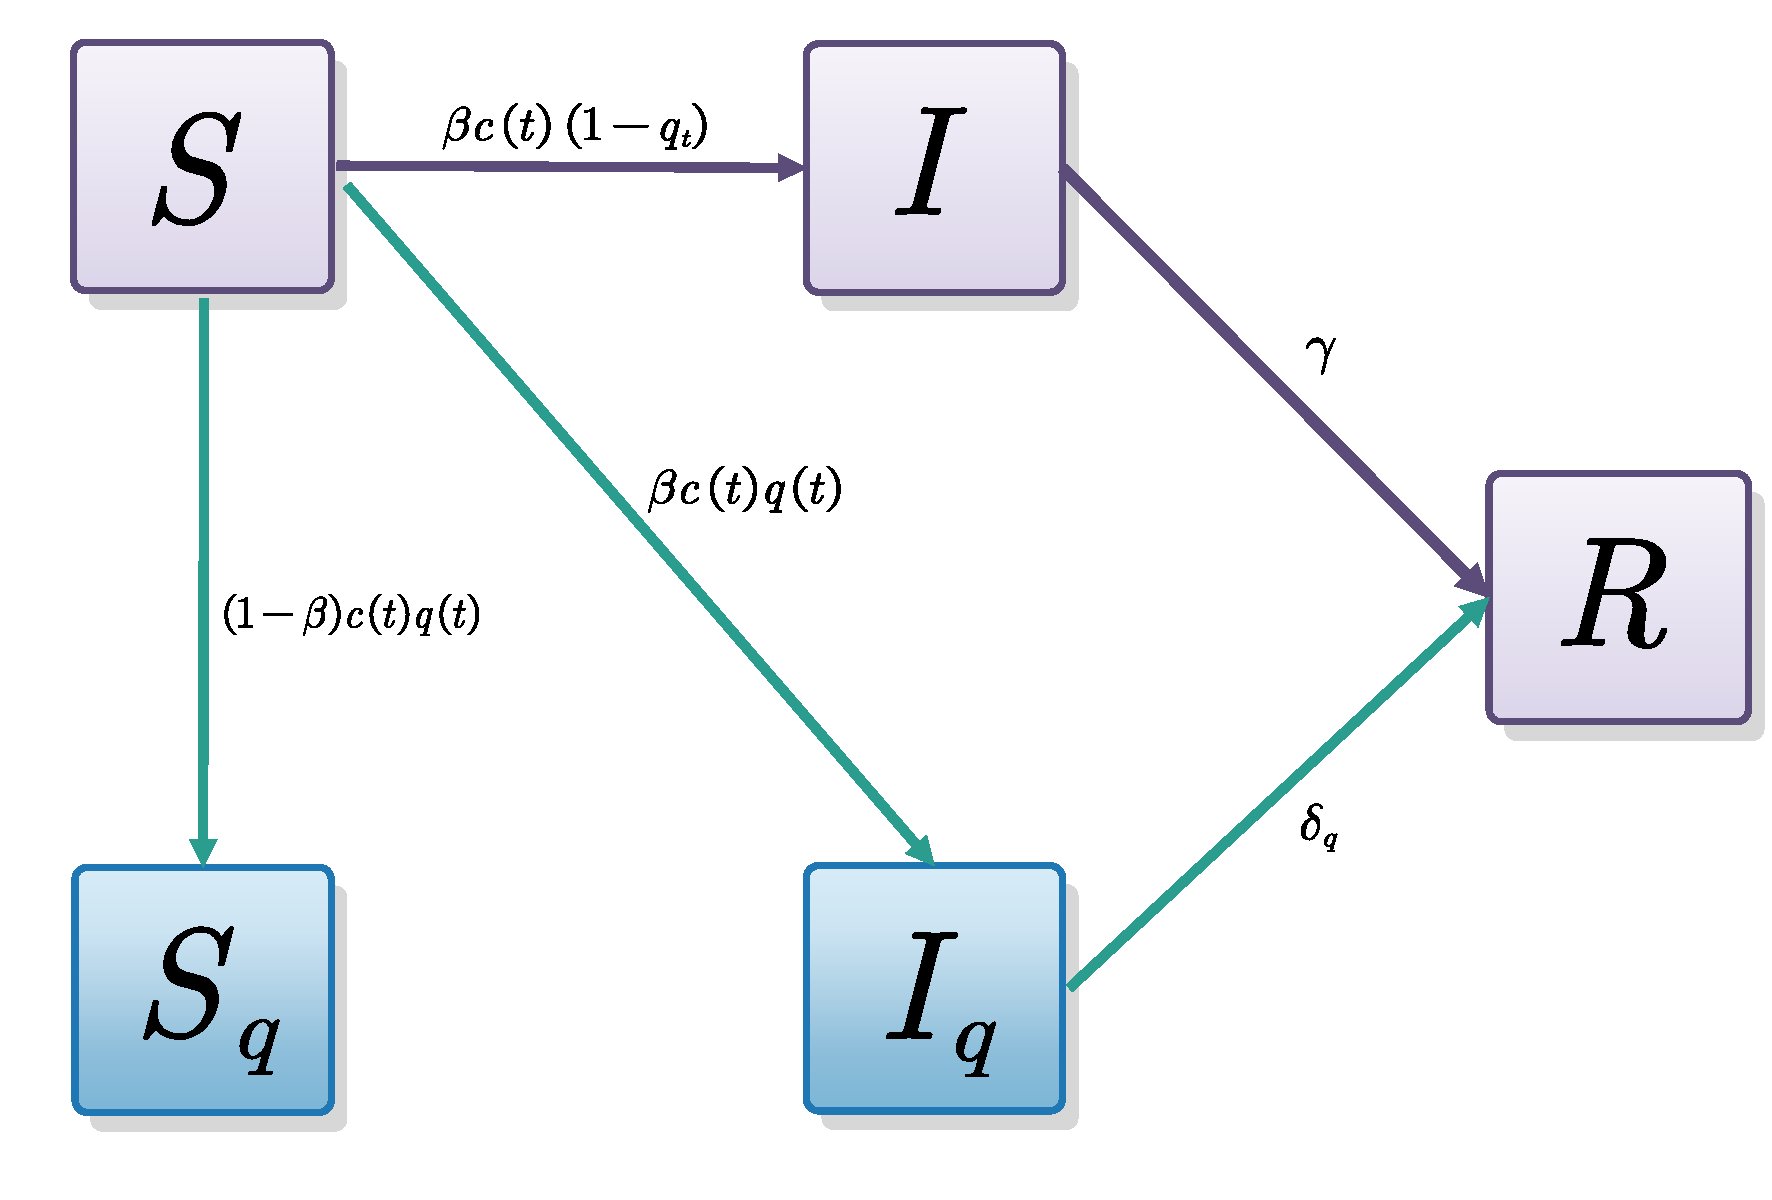
\includegraphics[width=0.7\textwidth]{figures/Fig1.pdf}
\caption{含接触追踪与隔离的 SIQR 型模型。$S,S_q,I,I_q,R$ 分别表示社区易感者、隔离易感者、非隔离感染者、隔离感染者和康复者。}
\label{fig:model_schematic}
\end{figure}

这一模型保留了文献\cite{Zhou2024SPCI}中社区传播与接触追踪的二维结构。以下假定 $N,c_0,\gamma,\delta_q>0$、$0<\beta\le1$、$0\le q_0<1$，初始仓室均非负且总和为 $N$，其中 $S_0,I_0>0$。人数以人为单位，$c,\gamma,\delta_q$ 的单位为时间的倒数，$\beta,q$ 为无量纲比例。文中沿用的“隔离率”指比例 $q$，不是检出感染者的连续时间风险率。

隔离者不参与社区传播，隔离易感者在研究时段内不返回 $S$；模型也不包括输入病例、出生和免疫丧失。在这些假设下，$S$ 的减少包含感染与未感染者隔离两部分，不能全部解释为感染后获得免疫。

\begin{proposition}
\label{prop:model:positive}
若 $c(t)\ge0$ 局部有界且可测，$q(t)\in[0,1]$ 可测，则式\eqref{eq:model:full}存在唯一全局绝对连续解，方程在几乎处处意义下成立。各仓室非负、总和恒为 $N$，且所有有限时刻均有 $S(t),I(t)>0$。
\end{proposition}
\begin{proof}
方程右端关于状态局部 Lipschitz，关于时间可测且在有界状态集上局部可积，故有唯一局部绝对连续解。前两式给出
\begin{align*}
S(t)&=S_0\exp\!\left[-\int_0^t\frac{c(s)[\beta+(1-\beta)q(s)]}{N}I(s)\,ds\right],\\
I(t)&=I_0\exp\!\left[\int_0^t\left(\frac{\beta c(s)(1-q(s))}{N}S(s)-\gamma\right)ds\right].
\end{align*}
隔离易感者的流入非负；隔离感染者由变参数公式保持非负；$\dot R\ge0$。五式相加得总人数守恒，因此所有分量有界，局部解可以延拓至任意有限时刻。上述指数表达式同时给出 $S,I$ 的严格正性。
\end{proof}

\subsection{感染上限、启动与退出条件}
\label{sec:model:strategy}
记 $\eta>0$ 为给定的社区非隔离感染人数上限，要求全过程满足 $I(t)\le\eta$，并记 $\theta=\eta/N$。该上限可参考医疗服务能力及防控目标选取\cite{Miclo2022ICU,Angulo2021}。本文将其作为外生参数，研究首次达到阈值后维持感染人数不变、并在满足退出条件时恢复常规控制的一类策略。

记常规控制为 $(c_0,q_0)$。当 $0<I_0<\eta$ 时，系统首先按常规控制演化。若常规感染峰值不超过 $\eta$，则无需为满足该上限加强干预；否则在感染人数首次上升至 $\eta$ 时启动，记该时刻为 $t_1$，并记 $S^*=S(t_1)$。本文规定控制期间满足
\begin{equation}
I(t)\equiv\eta,\qquad 0<c(t)\le c_0,\qquad q_0\le q(t)\le1,
\quad t_1\le t\le t_2.
\label{eq:model:plateau-requirement}
\end{equation}
这一阶段称为阈值控制期。由感染者方程，维持正的恒定感染人数要求
\begin{equation}
\frac{\beta c(t)(1-q(t))S(t)}{N}=\gamma.
\label{eq:model:balance}
\end{equation}
左端为单位非隔离感染者引起的新社区感染速率。固定 $c=c_0$ 时，该关系确定所需的隔离比例；允许 $c,q$ 同时调节时，它只规定两者必须共同满足的平衡。

常规控制下的临界易感者人数为
\begin{equation}
S_c=\frac{\gamma N}{\beta c_0(1-q_0)}.
\label{eq:model:Sc}
\end{equation}
本文规定 $t_2$ 为阈值控制期内首次达到 $S=S_c$ 的时刻，并在其后恢复 $(c_0,q_0)$。以下结果说明首次触发、维持阈值与上述退出条件各自的状态依据。

\Needspace{6\baselineskip}
\begin{proposition}
\label{prop:model:threshold-rationale}
设常规轨迹在有限时刻 $t_1$ 首次由下方到达 $I=\eta$，且 $S(t_1)=S^*>S_c$，则有以下结论。
\begin{enumerate}
\renewcommand{\labelenumi}{(\roman{enumi})}
\item 在首次加强干预之前采用 $(c_0,q_0)$ 的策略，若始终满足 $I\le\eta$，则首次加强干预的时刻不能晚于 $t_1$；常规轨迹在 $[0,t_1]$ 上满足该上限。
\item 在边界状态 $(S,\eta)$ 上，感染人数的瞬时导数非正当且仅当
\[
\frac{\beta c(1-q)S}{N}\le\gamma.
\]
若在一个时间区间内维持 $I=\eta$，则等号须几乎处处成立。
\item 从状态 $(S,\eta)$ 起恢复并保持 $(c_0,q_0)$，其后始终满足感染上限，当且仅当 $S\le S_c$。因此，沿任一从 $S^*>S_c$ 出发并持续维持 $I=\eta$ 的允许轨迹，首次达到 $S_c$ 是该轨迹上可以直接恢复常规控制的最早时刻。
\end{enumerate}
\end{proposition}
\begin{proof}
常规轨迹在首次到达时满足
\[
\dot I(t_1)=\eta\left[\frac{\beta c_0(1-q_0)S^*}{N}-\gamma\right]>0.
\]
若其后仍维持常规控制一段正时间，由连续性，感染人数会超过 $\eta$，故首次加强时刻不能晚于 $t_1$。在此之前不超过阈值则由首次到达的定义得到。

第二项直接由模型的感染者方程在 $I=\eta$ 时求得。对于有界可测时间控制，若 $I$ 在一个区间恒等于 $\eta$，则 $\dot I=0$ 几乎处处，故等号几乎处处成立。

恢复常规控制后有
\[
\dot I=\gamma I\left(\frac{S}{S_c}-1\right),\qquad
\dot S=-\frac{c_0[\beta+(1-\beta)q_0]}{N}SI<0.
\]
若恢复时 $S\le S_c$，此后 $S$ 严格下降，因而所有后续正时间均有 $\dot I<0$，感染人数不再超过 $\eta$。若恢复时 $S>S_c$，则恢复后的一个右邻域内有 $\dot I>0$，立即违反上限。阈值控制期内 $S$ 也严格下降，故沿该轨迹首次到达 $S_c$ 时即可恢复常规，而不能在此之前从阈值上直接退出。
\end{proof}

命题\ref{prop:model:threshold-rationale}中的最晚启动只相对于首次加强前未被改变的常规轨迹；最早退出只相对于已选定的恒定感染轨迹，不比较不同轨迹的退出时间。等式\eqref{eq:model:balance}表示感染增长恰好为零，既不唯一确定双控制分配，也不等于瞬时或累计成本最小。本文以这一规定过程作为研究对象，并不据此证明它在全部满足 $I\le\eta$ 的控制中最优。实施能力不足、观测误差或响应延迟存在时，可能需要提前干预或预留安全余量。

第\ref{sec:s1}--\ref{sec:s1:shape}节先固定 $c=c_0$，建立仅加强隔离的解析基准，并给出额外隔离能力上限下的实施判据；第\ref{sec:joint}节再允许两种控制同时变化，引入最低允许接触率 $c_{\min}$，考察两种能力限制下的可行分配。各策略在阈值控制期以外均采用相同的常规控制。第\ref{sec:joint}节的时间、感染和成本最优性均限定于相同进入与退出状态、始终保持 $I=\eta$ 的控制类，不比较提前干预、运行于 $I<\eta$ 或改变退出规则的方案。

\subsection{常规传播轨迹与触发条件}
$S,I$ 的方程不依赖其余仓室，因而启动与退出后的传播分析可归结为
\begin{equation}
\dot S=-\beta_1(t)SI,\qquad \dot I=\beta_2(t)SI-\gamma I.
\label{eq:model:reduced-si}
\end{equation}
其中
\begin{equation}
\beta_1(t)=\frac{c(t)[\beta+(1-\beta)q(t)]}{N},\qquad
\beta_2(t)=\frac{\beta c(t)(1-q(t))}{N}.
\label{eq:model:beta12-general}
\end{equation}
在常规阶段，记
\begin{equation}
\beta_1^0=\frac{c_0[\beta+q_0(1-\beta)]}{N},\quad
\beta_2^0=\frac{\beta c_0(1-q_0)}{N},\quad
\rho_1=\frac{\gamma}{\beta_1^0},\qquad
\frac{\beta_2^0}{\beta_1^0}=\frac{\rho_1}{S_c}.
\label{eq:model:beta12-baseline}
\end{equation}
消去时间或直接求导可得首次积分\cite{Zhou2024SPCI}
\begin{equation}
I(t)+\frac{\beta_2^0}{\beta_1^0}S(t)-\rho_1\ln S(t)=I_0+\frac{\beta_2^0}{\beta_1^0}S_0-\rho_1\ln S_0=:C_0,
\label{eq:model:first-integral}
\end{equation}
其中对数中的人数采用固定且统一的计数单位；后续计算均可写成人数比值。因此常规轨迹满足
\begin{equation}
I(S)=I_0+\frac{\beta_2^0}{\beta_1^0}(S_0-S)+\rho_1\ln\frac{S}{S_0}.
\label{eq:model:routine-orbit}
\end{equation}
当 $S_0\le S_c$ 时，所有 $t>0$ 均有 $I'(t)<0$，峰值为 $I_0$。当 $S_0>S_c$ 时，在 $S>S_c$ 的阶段有 $I\ge I_0$，从而 $\dot S\le-\beta_1^0 I_0S$，系统在有限时间到达 $S_c$。感染人数在该时刻由增转减，故常规峰值的完整表达为
\begin{equation}
I_{\max}^{no}=\begin{cases}
I_0,&S_0\le S_c,\\
I_0+\frac{\beta_2^0}{\beta_1^0}(S_0-S_c)+\rho_1\ln(S_c/S_0),&S_0>S_c.
\end{cases}
\label{eq:s1:Imax-no}
\end{equation}
以下关于正持续时间阈值控制的结果均在
\begin{equation}
S_0>S_c,\qquad 0<I_0<\eta<I_{\max}^{no}
\label{eq:model:trigger}
\end{equation}
下讨论。该条件保证常规传播会在达到峰值前触及感染上限。



\section{仅隔离控制的解析基准}
\label{sec:s1}
固定 $c=c_0$ 时，维持 $I=\eta$ 唯一确定隔离控制函数，启动状态、控制时长和累计新增感染均可由易感者轨迹表示。退出后恢复常规控制，感染人数继续下降，因此退出时刻与清零时间仍须分别计算。

\subsection{启动、控制轨迹与退出}
在条件\eqref{eq:model:trigger}下，常规轨迹先后两次经过 $I=\eta$，分别位于感染人数增加和减少的阶段。本文使用第一次交点。
\begin{theorem}
\label{thm:s1:start}\label{thm:s1:trigger}
设条件\eqref{eq:model:trigger}成立，并令
\begin{equation}
z_\eta=-\frac{1}{S_c}\exp\!\left[-\frac{C_0-\eta}{\rho_1}\right]
=-\frac{S_0}{S_c}\exp\!\left[-\frac{S_0}{S_c}+\frac{\eta-I_0}{\rho_1}\right].
\label{eq:s1:lambert-argument}
\end{equation}
则 $z_\eta\in(-e^{-1},0)$，唯一的启动状态及相应时间为
\begin{equation}
S^*=-S_cW_{-1}(z_\eta),\qquad S_c<S^*<S_0,
\label{eq:s1:Sstar-lambert}
\end{equation}
\begin{equation}
t_1=\frac{1}{\beta_1^0}\int_{S^*}^{S_0}
\frac{dS}{S[I_0+\frac{\beta_2^0}{\beta_1^0}(S_0-S)+\rho_1\ln(S/S_0)]}>0.
\label{eq:s1:t1}
\end{equation}
这里 $W_{-1}$ 为 Lambert $W$ 函数的下实分支。
\end{theorem}
\begin{proof}
将 $I=\eta$ 代入式\eqref{eq:model:first-integral}，得
$(-S/S_c)e^{-S/S_c}=z_\eta$。又由峰值公式，
\[
z_\eta=-e^{-1}\exp\!\left[-\frac{I_{\max}^{no}-\eta}{\rho_1}\right]\in(-e^{-1},0).
\]
在此区间，$W_0(z)\in(-1,0)$、$W_{-1}(z)<-1$\cite{Corless1996}。前者给出的状态小于 $S_c$，对应感染人数下降后的交点。由于式\eqref{eq:model:routine-orbit}在 $S\in(S_c,S_0)$ 上关于 $S$ 严格递减，且端点感染人数分别为 $I_{\max}^{no}$ 与 $I_0$，该区间恰有一个交点，须取 $W_{-1}$。沿常规易感者方程分离变量即得式\eqref{eq:s1:t1}；积分区间上 $I(S)\ge I_0>0$，所以 $t_1$ 有限。
\end{proof}
若 $\eta=I_0$，可取 $t_1=0,S^*=S_0$。若 $\eta=I_{\max}^{no}$，两交点合并为 $S_c$，控制时长为零。若 $\eta<I_0$，初始状态已不满足感染上限。

启动时有 $S^*>S_c$，常规隔离比例不足以阻止感染人数增加。为保持 $I=\eta$，需立即提高隔离比例，并随易感者减少而调整。记
\begin{equation}
\bar S=\frac{(1-\beta)\gamma N}{\beta c_0},\qquad
\frac{\bar S}{S_c}=(1-\beta)(1-q_0)<1.
\label{eq:s1:barS}
\end{equation}
\begin{theorem}
\label{thm:s1:qc-structure}\label{thm:s1:platform}
在条件\eqref{eq:model:trigger}下，固定 $c(t)=c_0$。阈值控制期内保持 $I(t)=\eta$ 所需的隔离比例唯一为
\begin{equation}
q_c(S)=1-\frac{\gamma N}{\beta c_0S},\qquad S_c\le S\le S^*.
\label{eq:s1:q-control}
\end{equation}
相应的状态轨迹和控制时长为
\begin{equation}
S(t)=\bar S+(S^*-\bar S)e^{-c_0\eta(t-t_1)/N},\qquad I(t)=\eta,
\label{eq:s1:S-analytic}
\end{equation}
\begin{equation}
\Delta t=t_2-t_1=\frac{N}{c_0\eta}\ln\frac{S^*-\bar S}{S_c-\bar S}.
\label{eq:s1:t2}
\end{equation}
以式\eqref{eq:s1:S-analytic}代入式\eqref{eq:s1:q-control}定义 $q_c(t)$，则完整控制为
\begin{equation}
c(t)=c_0,\qquad q(t)=\begin{cases}
q_0,&t<t_1,\\
q_c(t),&t_1\le t\le t_2,\\
q_0,&t>t_2.
\end{cases}
\label{eq:s1:q-piecewise}
\end{equation}
它满足 $I(t)\le\eta$ 对所有 $t\ge0$ 成立。
\end{theorem}
\begin{proof}
由 $I=\eta>0$ 和 $\dot I=0$，式\eqref{eq:model:balance}唯一解出式\eqref{eq:s1:q-control}。代入 $S$ 方程得
\[
\dot S=-\frac{c_0\eta}{N}(S-\bar S),\qquad S(t_1)=S^*,
\]
故有式\eqref{eq:s1:S-analytic}。由 $S^*>S_c>\bar S$，轨迹严格下降并在式\eqref{eq:s1:t2}给出的有限时间首次到达 $S_c$。该区间上 $q_c(S_c)=q_0$、$q_0\le q_c(S)<1$，控制满足界限。

反过来，将如此得到的时间函数 $q_c(t)$ 代回原方程，式\eqref{eq:s1:S-analytic}与 $I=\eta$ 满足前两个方程及启动初值，其余仓室由线性方程或积分确定。由命题\ref{prop:model:positive}的解唯一性，该控制确实实现恒定感染，而不只是形式上满足 $\dot I=0$。启动前 $I<\eta$；退出后 $S<S_c$，故 $\dot I<0$，全程不超过阈值。
\end{proof}

\begin{corollaryn}
\label{cor:s1:qc-structure}
上述控制在 $t_1$ 从 $q_0$ 跳升至
\begin{equation}
q_{\max}=1-\frac{\gamma N}{\beta c_0S^*}>q_0,
\label{eq:s1:qmax}
\end{equation}
在 $(t_1,t_2)$ 严格递减，并在 $t_2$ 连续恢复为 $q_0$。若另有追踪隔离比例的上限 $q_0\le q_{\rm cap}<1$，则上述仅隔离控制可实施，当且仅当
\[
q_{\max}\le q_{\rm cap}
\quad\Longleftrightarrow\quad
\frac{\beta c_0(1-q_{\rm cap})S^*}{N}\le\gamma.
\]
该条件成立时，能力限制不改变上述控制轨迹、控制时长及成本公式。
\end{corollaryn}
\begin{proof}
由于 $q_c(S)$ 关于 $S$ 严格增加，$S^*>S_c$ 给出启动跳跃。沿控制轨迹，
\begin{equation}
\frac{dq_c(t)}{dt}=-\frac{\gamma\eta}{\beta}
\frac{S(t)-\bar S}{S(t)^2}<0.
\label{eq:s1:qprime}
\end{equation}
又 $q_c(S_c)=q_0$，故退出时连续。控制比例的最大值在启动时取得，因此全时段的能力限制等价于检查这一最大值；由式\eqref{eq:s1:qmax}整理即得上述等价式。当 $q_{\rm cap}=q_{\max}$ 时，控制只在启动时恰好达到能力上限，随后严格低于上限。
\end{proof}
若 $q_{\rm cap}<q_{\max}$，则在规定启动状态取 $q=q_{\rm cap}$ 仍有 $\dot I>0$，截断原控制函数会使感染人数在启动后超过阈值。其他参数及 $q_{\rm cap}$ 固定时，命题\ref{prop:s1:sensitivity}表明提高触发区间内的阈值会降低 $q_{\max}$，保持已有的可行性。降低阈值则可能使所需隔离比例超过能力上限。

将式\eqref{eq:s1:S-analytic}代入式\eqref{eq:s1:q-control}，得到以启动或退出时刻为参照的时间开环控制：
\begin{equation}
\begin{split}
q_c(t)
&=1-\frac{1}{\left[\dfrac{\beta c_0S^*}{\gamma N}+\beta-1\right]
 e^{-c_0\eta(t-t_1)/N}+1-\beta}\\
&=1-\frac{1}{\left[\dfrac{q_0}{1-q_0}+\beta\right]
 e^{c_0\eta(t_2-t)/N}+1-\beta}.
\end{split}
\label{eq:s1:q-time-explicit}
\end{equation}
两种时间表达沿解析轨迹与式\eqref{eq:s1:q-control}等价，均由名义模型预先确定。感染人数偏离阈值后的纠偏不包含在这一控制函数中。三阶段数值轨迹见图\ref{fig:scenario1:single-sim}，具体数值在第\ref{sec:numerics}节的仅隔离基准比较中统一展示。

\subsection{退出后的动态与累计新增感染}
退出后的常规轨迹给出剩余易感者的极限，并在 $\eta>1$ 时确定清零时间。累计新增感染由启动前、阈值控制期和退出后三段的感染流入相加得到。
\begin{theorem}
\label{thm:s1:tend}\label{thm:s1:post}
从 $(S_c,\eta)$ 恢复常规控制后，$S(t)$ 和 $I(t)$ 对 $t>t_2$ 均严格递减，且
\begin{equation}
I(t)\to0,\qquad
S(t)\to S_\infty=-S_cW_0\!\left(-e^{-1-\eta/\rho_1}\right)\in(0,S_c).
\label{eq:s1:Sinfty}
\end{equation}
若 $\eta>1$，则唯一的 $t_{\rm end}>t_2$ 满足 $I(t_{\rm end})=1$、$I'(t_{\rm end})<0$。记 $S_{\rm end}=S(t_{\rm end})$，有
\begin{equation}
S_{\rm end}=-S_cW_0\!\left(-e^{-1-(\eta-1)/\rho_1}\right),
\label{eq:s1:Send}
\end{equation}
\begin{equation}
t_{\rm end}=t_2+\frac{1}{\beta_1^0}\int_{S_{\rm end}}^{S_c}
\frac{dS}{S[\eta+\frac{\beta_2^0}{\beta_1^0}(S_c-S)+\rho_1\ln(S/S_c)]}.
\label{eq:s1:tend}
\end{equation}
\end{theorem}
证明见附录\ref{sec:proof:post-dynamics}。
若 $\eta=1$，则 $I(t_2)=1$ 但 $I'(t_2)=0$，不属于上述终点定义。若 $\eta<1$，退出后始终 $I<1$，也不存在上述终点。由于 $\delta_q>0$ 且隔离感染仓室的输入趋于零，另有 $I_q(t)\to0$。$S_q,R$ 单调有界，因此也存在极限。

当 $\eta>1$ 时，按第\ref{sec:cost}节的定义，将分别进入 $I$ 和 $I_q$ 的累计新增感染合计为 $\Itcum$，统计至 $t_{\rm end}$。
\begin{theorem}
\label{thm:s1:Itcum}
在前述仅隔离控制下，若 $\eta>1$，则
\begin{equation}
\begin{split}
\Itcum={}&\frac{\beta}{\beta+q_0(1-\beta)}(S_0-S^*+S_c-S_{\rm end})\\
&+\beta\left[S^*-S_c+\bar S\ln\frac{S^*-\bar S}{S_c-\bar S}\right].
\end{split}
\label{eq:s1:cumulative}
\end{equation}
将 $S_{\rm end}$ 替换为 $S_\infty$，即得到计算至无限时刻的累计新增感染。
\end{theorem}
\begin{proof}
前后常规阶段均有
\[
\frac{\beta c_0SI}{N}=\frac{\beta}{\beta+q_0(1-\beta)}(-\dot S),
\]
所以两段积分分别由 $S_0-S^*$、$S_c-S_{\rm end}$ 给出。阈值控制期内使用 $dt=-N\,dS/[c_0\eta(S-\bar S)]$，得到
\[
\int_{t_1}^{t_2}\frac{\beta c_0S\eta}{N}\,dt
=\beta\int_{S_c}^{S^*}\frac{S}{S-\bar S}\,dS
=\beta\left[S^*-S_c+\bar S\ln\frac{S^*-\bar S}{S_c-\bar S}\right].
\]
三段相加即得结论；无穷时刻的表达由极限得到。
\end{proof}
\subsection{阈值与常规接触率的影响}
\label{sec:scaling-theory}
阈值与常规接触率都会改变启动状态，后者还改变退出状态。控制时长随阈值严格下降，但对常规接触率的变化方向不固定；求导时须同时计入 $S^*$ 和 $S_c$ 对参数的依赖。

除特别说明外，以下偏导数均固定 $N,S_0,I_0$ 及其余独立参数，并在相应触发条件的内部讨论。$\eta$ 作为独立设计参数；若它随其他参数同步调整，相应总变化应按复合函数求导。在 $q_0=0$ 或 $\beta=1$ 的边界，涉及该参数的导数理解为允许参数侧的单侧导数。$S_c,S_q,q_c$ 中的下标均按变量定义使用，不表示求导。

\begin{lemma}
\label{lem:s1:Sstar-sensitivity}
在条件\eqref{eq:model:trigger}下，启动状态满足
\begin{equation}
\frac{\partial S^*}{\partial\eta}<0,\qquad
\frac{\partial S^*}{\partial c_0}>0,\qquad
\frac{\partial S^*}{\partial\beta}>0,\qquad
\frac{\partial S^*}{\partial q_0}<0.
\label{eq:s1:Sstar-signs}
\end{equation}
\end{lemma}
证明见附录\ref{sec:proof:start-sensitivity}。

提高阈值使控制开始时的易感者人数减小，由此产生干预负担与累计新增感染之间的权衡。
\begin{proposition}
\label{prop:threshold-tradeoff}\label{prop:s1:sensitivity}
对于仅隔离控制，在触发区间内有
\begin{equation}
\frac{\partial t_1}{\partial\eta}>0,\quad
\frac{\partial q_{\max}}{\partial\eta}<0,\quad
\frac{\partial\Delta t}{\partial\eta}<0,\quad
\frac{\partial J_q}{\partial\eta}<0,\quad
\frac{\partial J}{\partial\eta}<0.
\label{eq:threshold-tradeoff}
\end{equation}
若进一步有 $\eta>1$，则 $\partial\Itcum/\partial\eta>0$。计算至无限时刻的累计新增感染也随 $\eta$ 严格增加。
\end{proposition}
证明见附录\ref{sec:proof:threshold-tradeoff}。
提高阈值降低所需最大隔离比例、控制时长和成本，但在 $\eta>1$ 时增加计算至清零终点的累计新增感染。清零时间还包括退出后的下降过程，其变化需结合式\eqref{eq:s1:tend}判断。

常规接触率的比较须先确定触发范围。固定其余参数，当
\[
c_0\le\frac{\gamma N}{\beta(1-q_0)S_0}
\]
时，常规峰值为 $I_0$；超过该值后，式\eqref{eq:s1:Imax-no}给出
\begin{equation}
\frac{dI_{\max}^{no}}{dc_0}
=-\frac{\rho_1}{c_0}\ln\frac{S_c}{S_0}>0.
\label{eq:s1:Imax-no-c0-derivative}
\end{equation}
此时峰值从 $I_0$ 严格增加至 $I_0+\beta_2^0 S_0/\beta_1^0$。若
\[
I_0<\eta<I_0+\frac{\beta_2^0}{\beta_1^0}S_0,
\]
则唯一的临界常规接触率 $c_{0,\min}(\eta)$ 满足
\begin{equation}
I_{\max}^{no}\bigl(c_{0,\min}(\eta)\bigr)=\eta,
\qquad c_{0,\min}(\eta)>\frac{\gamma N}{\beta(1-q_0)S_0}.
\label{eq:s1:c0-min-def}
\end{equation}
正控制时长恰在 $c_0>c_{0,\min}(\eta)$ 时出现。

\begin{proposition}
\label{prop:contact-effects}\label{cor:s1:duration-sensitivity}
在触发条件内部，对于仅隔离控制，
\[
\frac{\partial t_1}{\partial c_0}<0,\qquad
\frac{\partial q_{\max}}{\partial c_0}>0,\qquad
\frac{\partial\Delta t}{\partial\beta}>0,\qquad
\frac{\partial\Delta t}{\partial q_0}<0.
\]
接触率对控制时长的影响由
\begin{equation}
\frac{\partial\Delta t}{\partial c_0}
=\frac{N}{c_0^2\eta}
\left\{\frac{S^*}{S^*-\bar S}
\left[1+\frac{S_c}{S^*-S_c}\ln\frac{S_0}{S^*}\right]
-\ln\frac{S^*-\bar S}{S_c-\bar S}\right\}
\label{eq:duration-c0}
\end{equation}
确定，其符号不能统一为正或负。固定 $I_0<\eta<I_0+\beta_2^0S_0/\beta_1^0$ 时，$\Delta t$ 在 $c_0\in(c_{0,\min},\infty)$ 内至少有一个极大值，但不据此断言极大值唯一。
\end{proposition}
证明见附录\ref{sec:proof:contact-effects}。
式\eqref{eq:duration-c0}的等价符号判据为
\begin{equation}
\frac{\partial\Delta t}{\partial c_0}\gtrless0
\quad\Longleftrightarrow\quad
\ln\frac{S_0}{S^*}\gtrless
\frac{S^*-S_c}{S_c}
\left[\frac{S^*-\bar S}{S^*}\ln\frac{S^*-\bar S}{S_c-\bar S}-1\right],
\label{eq:duration-c0-equivalent}
\end{equation}
等号亦相应成立。右端非正时，$\partial\Delta t/\partial c_0>0$。

较高接触率使干预更早启动并要求更大的隔离比例，控制时长则由起止状态与时间尺度共同决定，因而可以向两个方向变化。

人口规模的比较还取决于初值与阈值的缩放方式。记 $s=S/N,i=I/N,\theta=\eta/N$，以下固定归一化初值；固定绝对初始感染人数或固定绝对阈值时，比较条件不同。
\begin{proposition}
\label{prop:scaling}
对于仅隔离控制，固定 $s_0,i_0$ 和 $\beta,\gamma,c_0,q_0$。在阈值控制被触发时，$t_1,\Delta t,q_{\max},J$ 以及存在内部拐点时的 $\lambda$ 对 $N,\eta$ 的依赖仅通过 $\theta=\eta/N$ 表现。最终累计新增感染除以 $N$ 后亦不依赖 $N$。但是，使用绝对终点 $I=1$ 时，$t_{\rm end}$ 及计算至该终点的累计新增感染比例一般仍含 $N$。
\end{proposition}
\begin{proof}
常规阶段的归一化系统为
\[
\dot s=-c_0[\beta+q_0(1-\beta)]si,\qquad
\dot i=[\beta c_0(1-q_0)s-\gamma]i.
\]
它不含 $N$，触发条件为 $i=\theta$，所以 $t_1$ 与 $s^*=S^*/N$ 仅依赖上述固定量和 $\theta$。又
\[
s_c=\frac{\gamma}{\beta c_0(1-q_0)},\qquad
\bar s=\frac{(1-\beta)\gamma}{\beta c_0},\qquad
\Delta t=\frac1{c_0\theta}\ln\frac{s^*-\bar s}{s_c-\bar s}.
\]
例如，二次成本的归一化表达为
\begin{equation}
J=\frac{2}{c_0\theta}\int_{s_c}^{s^*}
\frac{(1-s_c/s)^2}{s-\bar s}\,ds,
\label{eq:dom:Jtheta}
\end{equation}
其中仅含归一化状态和固定参数。代入控制表达可得其余结论。无限时间的终点为 $i\to0$，同样不含 $N$；有限的操作性终点却为 $i=1/N$，因而保留绝对人口尺度。
\end{proof}

小初值与低阈值的联合极限，以及固定正初值下的有限极限见补充材料第\ref{sec:sup:baseline-scan}节，完整参数扫描也列于该节。
\subsection{隔离比例的时间形态}
\label{sec:s1:shape}
仅隔离控制的隔离比例严格下降，其下降速度在存在内部拐点时达到唯一最大值。以下在 $c=c_0$ 下确定这一时刻及其在控制期内的相对位置。

\begin{theorem}
\label{thm:s1:inflection}
在条件\eqref{eq:model:trigger}下，$q_c(t)$ 在 $(t_1,t_2)$ 内存在唯一拐点，当且仅当
\begin{equation}
S_c<2\bar S<S^*,
\label{eq:s1:inflection-condition}
\end{equation}
等价地，$\frac12<(1-\beta)(1-q_0)<-\frac12W_{-1}(z_\eta)$。
内部拐点存在时，
\begin{equation}
S(t_{\rm inf})=2\bar S,\quad
 t_{\rm inf}=t_1+\frac{N}{c_0\eta}\ln\frac{S^*-\bar S}{\bar S},\quad
\qinf=1-\frac1{2(1-\beta)}.
\label{eq:s1:inflection-values}
\end{equation}
此时 $q_0<\qinf<q_{\max}$，且隔离比例的下降速度在 $t_{\rm inf}$ 唯一达到最大值。
\end{theorem}
\begin{proof}
对式\eqref{eq:s1:qprime}求导，得
\begin{equation}
\frac{d^2q_c(t)}{dt^2}
=\frac{\gamma c_0\eta^2}{\beta N}
\frac{(S-\bar S)(2\bar S-S)}{S^3}.
\label{eq:s1:qsecond}
\end{equation}
由于 $S>\bar S$，其符号由 $2\bar S-S$ 决定。$S$ 从 $S^*$ 严格下降至 $S_c$，所以恰在式\eqref{eq:s1:inflection-condition}成立时穿过 $2\bar S$，且只穿过一次。将该状态代入式\eqref{eq:s1:S-analytic}及\eqref{eq:s1:q-control}，即得时间和隔离比例。条件\eqref{eq:s1:inflection-condition}蕴含 $\beta<1/2$，故所列 $\qinf$ 表达式有定义。二阶导数先负后正，而一阶导数始终为负，故 $|dq_c/dt|$ 在该时刻达到唯一最大值。
\end{proof}

内部拐点存在时，其隔离比例只依赖 $\beta$。拐点在控制期内的相对位置为
\begin{equation}
\lambda=\frac{t_{\rm inf}-t_1}{t_2-t_1}
=\frac{\ln[(S^*-\bar S)/\bar S]}
{\ln[(S^*-\bar S)/(S_c-\bar S)]}\in(0,1).
\label{eq:s1:lambda}
\end{equation}
其中拐点前、后的两段时长分别为
\begin{equation}
t_{\rm inf}-t_1=\frac{N}{c_0\eta}\ln\frac{S^*-\bar S}{\bar S},\qquad
 t_2-t_{\rm inf}=\frac{N}{c_0\eta}\ln\frac{\bar S}{S_c-\bar S}.
\label{eq:s1:seg-high}
\end{equation}
$\lambda$ 是拐点前时长占控制时长的比例，数值越大，下降最快的时刻在控制期内越靠后。绝对时刻 $t_{\rm inf}$ 还取决于启动时刻和控制时长。

若 $2\bar S\le S_c$，则 $q_c''(t)<0$ 对 $t\in(t_1,t_2)$ 成立；等号对应拐点到达控制终点。若 $2\bar S\ge S^*$，则 $q_c''(t)>0$ 对 $t\in(t_1,t_2)$ 成立；等号对应拐点到达控制起点。两种等号情形均无内部拐点。特别地，$\beta=1$ 时 $\bar S=0$，始终不存在内部拐点。

相对位置的辅助导数、正负导数构造及数值结果见补充材料第\ref{sec:sup:inflection}节。各参数敏感性的成立条件汇总于附录\ref{sec:appendix:proofs}的表\ref{tab:sensitivity}。

\section{联合阈值控制的可行性与指标权衡}
\label{sec:joint}
维持 $I=\eta$ 只约束接触率与未被隔离比例的乘积，允许两种干预有不同分配。将这些分配用易感者状态参数化后，能力限制确定允许区间，控制时长则联系累计新增感染与新增隔离易感者人数。

\subsection{状态参数化与能力条件}
阈值控制期内 $S$ 严格下降，因而可以用 $S$ 参数化全部允许分配。沿用第\ref{sec:model:control-class}节的可测控制约定，以下对应均在几乎处处相等意义下成立。
记接触率和隔离比例的状态表达为 $c_c(S),q_c(S)$，对应的时间函数为 $c(t)=c_c(S(t))$、$q(t)=q_c(S(t))$。仅隔离控制对应 $c_c(S)\equiv c_0$。
\begin{theorem}
\label{thm:joint:representation}
规定的联合阈值控制与满足
\begin{equation}
\frac{c_0S_c}{S}\le c_c(S)\le c_0,\qquad S\in[S_c,S^*],
\label{eq:joint:contact-range}
\end{equation}
的有界可测函数相对应。隔离比例由
\begin{equation}
q_c(S)=1-\frac{\gamma N}{\beta c_c(S)S}
      =1-\frac{c_0(1-q_0)S_c}{c_c(S)S}
\label{eq:joint:q}
\end{equation}
确定，状态轨迹与控制时长满足
\begin{align}
t-t_1&=\frac{N}{\eta}\int_{S(t)}^{S^*}
\frac{du}{c_c(u)u-c_0\bar S},\label{eq:joint:time}\\
\Delta t[c_c]&=\frac{N}{\eta}\int_{S_c}^{S^*}
\frac{dS}{c_c(S)S-c_0\bar S}.\label{eq:joint:duration}
\end{align}
式\eqref{eq:joint:time}唯一确定严格递减的 $S(t)$。选取满足式\eqref{eq:joint:contact-range}的逐点代表后，退出时 $c(t)\to c_0$、$q(t)\to q_0$；若 $c_c(S)$ 连续，则两控制在阈值控制期内部连续。
\end{theorem}
证明见附录\ref{sec:proof:representation}。

选择 $c_c(S)$ 后，隔离比例、时间轨迹和控制时长随之确定。第\ref{sec:model:control-class}节的能力限制进一步将接触率约束为式\eqref{eq:joint:bounds}的区间。

\begin{corollaryn}
\label{cor:joint:feasibility}
上述能力限制等价于 $\underline c(S)\le c_c(S)\le\overline c(S)$。从 $S^*$ 至 $S_c$ 的整段阈值控制可行，当且仅当
\begin{equation}
\frac{\beta c_{\min}(1-q_{\rm cap})S^*}{N}\le\gamma.
\label{eq:joint:feasibility}
\end{equation}
利用式\eqref{eq:s1:qmax}，该条件也可写为
\[
c_{\min}(1-q_{\rm cap})\le c_0(1-q_{\max}).
\]
\end{corollaryn}
\begin{proof}
$c_c\ge c_{\min}$ 与式\eqref{eq:joint:contact-range}给出下界；由式\eqref{eq:joint:q}中的 $q_c\le q_{\rm cap}$ 得到上界。在 $S\in[S_c,S^*]$ 上，已有 $c_0S_c/S\le c_0$、$c_0S_c/S\le c_0(1-q_0)S_c/[(1-q_{\rm cap})S]$ 及 $c_{\min}\le c_0$，故只需检验
\[
c_{\min}\le\frac{c_0(1-q_0)S_c}{(1-q_{\rm cap})S}.
\]
其最严格处为 $S=S^*$，即式\eqref{eq:joint:feasibility}。条件成立时取 $c_c=(\underline c+\overline c)/2$，由前一定理得到可行控制；条件不成立时，启动状态附近不存在允许分配。
\end{proof}
由于 $c_{\min}\le c_0$，联合可行条件不强于仅隔离控制的条件，两者在 $c_{\min}=c_0$ 时相同。若 $q_{\rm cap}\ge q_{\max}$，两类控制均可行。若 $q_{\rm cap}<q_{\max}$ 而式\eqref{eq:joint:feasibility}成立，则接触减少补足仅隔离控制所缺的能力。后一情形下，沿用满足界限的逐点代表，由式\eqref{eq:joint:bounds}可知，在
\[
\frac{\gamma N}{\beta c_0(1-q_{\rm cap})}<S\le S^*
\]
上必须有 $c_c(S)<c_0$。接触减少至少在启动后的一段正时间内是必要的，这不要求隔离比例也必须高于 $q_0$。当 $S$ 降至上述区间下界及其以下时，仅隔离控制重新成为允许分配，是否采用它还取决于成本等目标。

若式\eqref{eq:joint:feasibility}不成立，首次触发状态附近不存在允许分配，按当前常规轨迹等到 $I=\eta$ 才启动的方案不可行。提前干预会改变启动状态，其可行性需另行分析。Angulo 等\cite{Angulo2021}在 SIR 模型中讨论了能力有限时需要提前启动的情形，但这一结果不直接保证本文 SIQR 模型中的提前干预可行。

由引理\ref{lem:s1:Sstar-sensitivity}，$S^*$ 随 $\eta$ 严格下降。因此，其余参数和能力界限固定时，某一内部阈值可行即保证所有更高且仍触发控制的阈值可行。降低感染上限还可能使启动时所需干预超过能力限制。

\subsection{显式策略族}
常数分配参数 $\alpha\in[0,1]$ 给出一个显式子族，连续连接两种单控制。取
\begin{align}
c_c(S;\alpha)&=c_0\left[\alpha+(1-\alpha)\frac{S_c}{S}\right],\label{eq:joint:explicit-c}\\
q_c(S;\alpha)&=1-\frac{(1-q_0)S_c}{S_c+\alpha(S-S_c)}.
\label{eq:joint:explicit-q}
\end{align}
式\eqref{eq:joint:explicit-c}满足\eqref{eq:joint:contact-range}。这里 $\alpha$ 表示干预分配，$\theta=\eta/N$ 和 $\lambda$ 分别保留阈值比例与拐点相对位置的含义。
\begin{theorem}
\label{thm:joint:explicit}
固定 $0<\alpha\le1$ 时，式\eqref{eq:joint:explicit-c}--\eqref{eq:joint:explicit-q}对应的阈值控制期状态为
\begin{equation}
S(t)=S_c+
\left(S^*-S_c+\frac{S_c-\bar S}{\alpha}\right)
 e^{-\frac{c_0\eta\alpha}{N}(t-t_1)}
-\frac{S_c-\bar S}{\alpha},\qquad I(t)=\eta,
\label{eq:joint:explicit-S}
\end{equation}
控制时长为
\begin{equation}
\Delta t(\alpha)=\frac{N}{c_0\eta\alpha}
\ln\!\left(1+\frac{\alpha(S^*-S_c)}{S_c-\bar S}\right).
\label{eq:joint:explicit-duration}
\end{equation}
$\alpha=0$ 时，相应表达为
\begin{equation}
S(t)=S^*-\frac{c_0\eta}{N}(S_c-\bar S)(t-t_1),\qquad
\Delta t(0)=\frac{N(S^*-S_c)}{c_0\eta(S_c-\bar S)}.
\label{eq:joint:explicit-zero}
\end{equation}
将上述 $S(t)$ 代入式\eqref{eq:joint:explicit-c}--\eqref{eq:joint:explicit-q}，即得到两个控制的时间表达。$\alpha=0$ 对应仅减少接触，$\alpha=1$ 恢复第\ref{sec:s1}节的仅隔离控制。对于 $0<\alpha<1$，阈值控制期内接触率严格增加、隔离比例严格下降，并在退出时同时连续恢复为 $(c_0,q_0)$。
\end{theorem}
\begin{proof}
代入式\eqref{eq:joint:Sdot}得
\[
\dot S=-\frac{c_0\eta}{N}\bigl[S_c-\bar S+\alpha(S-S_c)\bigr],
\qquad S(t_1)=S^*.
\]
分别求解 $\alpha>0$ 和 $\alpha=0$ 的线性方程，得到状态表达；令 $S(t_2)=S_c$ 得到控制时长。两组公式在 $\alpha\downarrow0$ 时连续衔接。对于 $0<\alpha<1$，
\[
\frac{\partial c_c(S;\alpha)}{\partial S}
=-\frac{c_0(1-\alpha)S_c}{S^2}<0,\qquad
\frac{\partial q_c(S;\alpha)}{\partial S}
=\frac{(1-q_0)S_c\alpha}{[S_c+\alpha(S-S_c)]^2}>0.
\]
结合 $\dot S<0$，得到时间单调性。代入 $S=S_c$ 得到退出值；代入 $\alpha=0,1$ 分别恢复两种单控制。
\end{proof}
控制启动时，$0<\alpha<1$ 的策略使 $c$ 向下跳跃、$q$ 向上跳跃。由于 $S^*>S_c$ 时常规控制不满足式\eqref{eq:joint:balance}，这一跳跃与退出时的连续恢复不同。
\begin{corollaryn}
\label{cor:joint:allocation-range}
在式\eqref{eq:joint:bounds}的能力限制下，上述显式族可行当且仅当
\begin{equation}
\max\!\left\{0,\frac{c_{\min}S^*-c_0S_c}{c_0(S^*-S_c)}\right\}
\le\alpha\le
\min\!\left\{1,\frac{S_c(q_{\rm cap}-q_0)}{(1-q_{\rm cap})(S^*-S_c)}\right\}.
\label{eq:joint:allocation-range}
\end{equation}
该区间非空当且仅当式\eqref{eq:joint:feasibility}成立。
\end{corollaryn}
\begin{proof}
显式族中 $c$ 不减、$q$ 不增，故只需在 $S=S^*$ 处检查 $c\ge c_{\min}$ 和 $q\le q_{\rm cap}$。代入式\eqref{eq:joint:explicit-c}--\eqref{eq:joint:explicit-q}并与 $\alpha\in[0,1]$ 取交，得到式\eqref{eq:joint:allocation-range}。未截断的下界不超过 $1$，未截断的上界非负；二者的大小关系等价于
$c_{\min}S^*\le c_0(1-q_0)S_c/(1-q_{\rm cap})$。
这正是式\eqref{eq:joint:feasibility}，故该区间与完整控制类同时非空。
\end{proof}
显式子族与完整控制类具有相同的非空条件。以下指标比较及第\ref{sec:joint:cost}节的成本最小化均考察全部允许的 $c_c(S)$。

\subsection{控制时长、累计新增感染与隔离人数}
固定进入与退出的二维状态 $(S^*,\eta)$ 和 $(S_c,\eta)$ 后，较大的 $c_c(S)$ 使 $S$ 下降更快。控制时长由式\eqref{eq:joint:duration}比较，控制期累计新增感染与新增隔离易感者人数则由以下恒等式联系。
\begin{theorem}
\label{thm:joint:comparison}
若两个允许控制的状态函数满足 $c_c^{(1)}(S)\ge c_c^{(2)}(S)$ 几乎处处成立，则
$\Delta t[c_c^{(1)}]\le\Delta t[c_c^{(2)}]$。若前一不等式在正测度集合上严格成立，则后一不等式严格。特别地，
\begin{equation}
\frac{N}{c_0\eta}\ln\frac{S^*-\bar S}{S_c-\bar S}
\le\Delta t[c_c]\le
\frac{N(S^*-S_c)}{c_0\eta(S_c-\bar S)}.
\label{eq:joint:duration-bounds}
\end{equation}
左侧等号当且仅当 $c_c(S)=c_0$ 几乎处处，即仅隔离控制；右侧等号当且仅当 $c_c(S)=c_0S_c/S$ 几乎处处，即仅减少接触。显式族的 $\Delta t(\alpha)$ 在 $[0,1]$ 上严格递减。

沿任一允许控制，其阈值控制期累计新增感染与新增隔离易感者人数分别满足
\begin{align}
\Itcum(t_2)-\Itcum(t_1)
&=\beta(S^*-S_c)+\gamma\eta(1-\beta)\Delta t,
\label{eq:joint:cumulative}\\
S_q(t_2)-S_q(t_1)
&=(1-\beta)\bigl[S^*-S_c-\gamma\eta\Delta t\bigr].
\label{eq:joint:quarantine}
\end{align}
当 $0<\beta<1$ 时，阈值控制期累计新增感染与控制时长具有相同排序，新增隔离易感者人数的排序相反；$\beta=1$ 时，累计新增感染均为 $S^*-S_c$，隔离易感者人数不增加。
\end{theorem}
\begin{proof}
式\eqref{eq:joint:duration}的被积函数关于 $c_c(S)$ 严格递减，故得到一般排序。由式\eqref{eq:joint:contact-range}又有
\[
\frac1{c_0(S-\bar S)}\le
\frac1{c_c(S)S-c_0\bar S}\le
\frac1{c_0(S_c-\bar S)}.
\]
积分给出两界。等号成立要求相应非负积分差为零，即两个状态函数几乎处处相等。显式族中 $c_c(S;\alpha)$ 对 $S>S_c$ 随 $\alpha$ 严格增加，故其控制时长严格减少。

积分式\eqref{eq:joint:Sdot}，得
\[
S^*-S_c=\frac{\eta}{N}\int_{t_1}^{t_2}c(t)S(t)\,dt
-\frac{c_0\eta\bar S}{N}\Delta t.
\]
左式积分项乘以 $\beta$ 即为阈值控制期总新增感染。由 $\beta c_0\bar S/N=\gamma(1-\beta)$，得到式\eqref{eq:joint:cumulative}。阈值控制期离开 $S$ 的人群分为新感染者与未感染的隔离者，故
\[
S^*-S_c=\Itcum(t_2)-\Itcum(t_1)+S_q(t_2)-S_q(t_1),
\]
代入前式得到式\eqref{eq:joint:quarantine}。
\end{proof}
无额外能力限制时，仅隔离控制使控制时长最短，并在 $0<\beta<1$ 时使阈值控制期累计新增感染最少、新增隔离易感者人数最多。其机制是未感染者隔离加快社区易感者的减少，这里计量的隔离人数不同于隔离人天。

加入能力限制后，两种单控制可能不再可行，可达到的时长端点由实际允许区间 $[\underline c(S),\overline c(S)]$ 确定。
\begin{corollaryn}
\label{cor:joint:capped-comparison}
若式\eqref{eq:joint:feasibility}成立，则
\begin{equation}
\Delta t[\overline c]\le\Delta t[c_c]\le\Delta t[\underline c],
\label{eq:joint:capped-duration}
\end{equation}
其中两端由式\eqref{eq:joint:duration}分别代入 $\overline c(S)$、$\underline c(S)$ 计算，且均可达到。达到左、右等号分别要求 $c_c=\overline c$、$c_c=\underline c$ 几乎处处成立。$0<\beta<1$ 时，同一两个控制分别达到受限类内最少和最多的阈值控制期累计新增感染。
\end{corollaryn}
\begin{proof}
在式\eqref{eq:joint:duration}中用 $\underline c\le c_c\le\overline c$ 比较即可。两个边界函数连续且满足限制，因而确实对应可行控制。感染量结论由式\eqref{eq:joint:cumulative}得到。
\end{proof}

全过程比较采用相同完整初值、共同的首次触发规则与二维退出状态 $(S_c,\eta)$。启动前和退出后均采用常规控制时，前后两段的共同贡献可从指标差中消去。
\begin{corollaryn}
\label{cor:joint:whole-epidemic}
设两种允许策略在启动前及退出后均采用 $(c_0,q_0)$，并从同一初始状态首次到达同一阈值 $\eta>1$。则
\begin{align}
t_{\rm end}^{(1)}-t_{\rm end}^{(2)}
&=\Delta t^{(1)}-\Delta t^{(2)},\label{eq:joint:whole-time}\\
\Itcum^{(1)}-\Itcum^{(2)}
&=\gamma\eta(1-\beta)\bigl(\Delta t^{(1)}-\Delta t^{(2)}\bigr).
\label{eq:joint:whole-cumulative}
\end{align}
第二式对计算至无限时刻的累计新增感染同样成立。能力限制下，$\overline c(S)$ 因而同时达到最短控制时长、最早社区清零时间；当 $0<\beta<1$ 时，也达到最少的全过程累计新增感染。
\end{corollaryn}
\begin{proof}
控制前两条轨迹相同，故 $t_1,S^*$ 相同。退出时的二维状态均为 $(S_c,\eta)$，由常规系统解的唯一性，退出后的 $S,I$ 轨迹只相差时间平移。因此，两种策略从退出到 $I=1$ 所需的时间相同，退出后的新增感染积分也相同。分别消去两策略共同的前后两段，再用式\eqref{eq:joint:cumulative}，得到所列等式。其余仓室在退出时可以不同，故这里不推断隔离感染者或医疗占用也具有相同轨迹。
\end{proof}

若式\eqref{eq:joint:feasibility}成立，每一个处于
$[\Delta t[\overline c],\Delta t[\underline c]]$ 内的控制时长都可实现。事实上，取
$c_c(S)=(1-x)\underline c(S)+x\overline c(S)$、$x\in[0,1]$，式\eqref{eq:joint:duration}连续地连接两端；若两界并非几乎处处相等，则该控制时长随 $x$ 严格下降。结合推论\ref{cor:joint:whole-epidemic}，在同一完整初值、阈值 $\eta>1$ 和前后常规控制下，若只对控制时长、清零时间和累计新增感染施加上限，则存在可行策略当且仅当最快控制 $\overline c$ 满足这些上限。成本上限须另行检验，因为最短控制时长与最小成本对应的控制未必相同。


\subsection{常规退出要求产生的感染下界}
在模型\eqref{eq:model:full}中，易感者的减少由感染与未感染者隔离共同造成。规定在有限时刻达到 $S=S_c$，会对累计新增感染产生不依赖具体分配的下界。
\begin{proposition}
\label{prop:exit-infection-lower-bound}
对于模型\eqref{eq:model:full}，若 $0\le q(t)\le1$、$c(t)\ge0$，且某一有限时刻 $T$ 满足 $S(T)=S_c<S_0$，则
\begin{equation}
\Itcum(T)\ge\beta(S_0-S_c).
\label{eq:exit-infection-lower-bound}
\end{equation}
若整个 $[0,T]$ 上另有 $q(t)\le q_{\rm cap}<1$，则
\begin{equation}
\Itcum(T)\ge
\frac{\beta}{\beta+(1-\beta)q_{\rm cap}}(S_0-S_c).
\label{eq:exit-infection-capped}
\end{equation}
\end{proposition}
\begin{proof}
由易感者方程和累计新增感染的定义，
\[
\frac{d\Itcum}{dt}
=\frac{\beta}{\beta+(1-\beta)q(t)}(-\dot S).
\]
$-\dot S\ge0$，且比例系数分别不小于 $\beta$ 和
$\beta/[\beta+(1-\beta)q_{\rm cap}]$。在 $[0,T]$ 上积分即得两式。
\end{proof}
这些界适用于本模型中要求有限时刻达到 $S_c$ 的控制任务，下界能否达到还取决于控制与能力约束。较低感染峰值、较少累计新增感染与这一退出要求可能不相容，仅重新分配两种干预不能消除该限制。


\section{二次成本下的最优分配}
\label{sec:joint:cost}
\subsection{状态积分与最小值存在性}
二次成本最小化同时考虑干预强度与控制时长，可由逐状态最小化的可测选择实现。控制时长最短的分配未必使式\eqref{eq:cost:J}最小，因为接触减少与追踪隔离的强度代价不同。由式\eqref{eq:joint:q}和式\eqref{eq:joint:time}的时间变换，成本写为接触率状态函数的积分：
\begin{equation}
J[c_c]=\frac{N}{\eta}\int_{S_c}^{S^*}f(S,c_c(S))\,dS,
\label{eq:joint:cost}
\end{equation}
其中
\begin{equation}
f(S,c)=
\frac{(1-c/c_0)^2+2\left(1-\dfrac{c_0S_c}{cS}\right)^2}
{cS-c_0\bar S}.
\label{eq:joint:cost-integrand}
\end{equation}
式\eqref{eq:joint:cost-integrand}采用默认权重 $1,2$。讨论一般正权重时，将分子中两项的系数分别替换为 $w_c,w_q$，并沿用 $f$ 的记号。
这里的 $c$ 是固定状态 $S$ 上待比较的接触率取值。式\eqref{eq:joint:Sdot}给出的易感者下降速度含有分母中的因子 $cS-c_0\bar S$。因此，$\frac{N}{\eta}f(S,c)$ 表示单位社区易感者减少量对应的成本，同时计入干预强度和相应的时间消耗。

有能力限制时使用式\eqref{eq:joint:bounds}的上下界，无额外限制时取 $\underline c(S)=c_0S_c/S$、$\overline c(S)=c_0$。以下分别在 $\mathcal A(\eta;c_{\min},q_{\rm cap})$ 或 $\mathcal A(\eta)$ 中最小化成本，假定整段允许区间非空，且不增加总时长、调整次数或控制变化率等约束。
\begin{theorem}
\label{thm:joint:cost-minimum}
在规定的全部有界可测阈值控制中，二次成本最小值可达到，且
\begin{equation}
\min_{c_c}J[c_c]
=\frac{N}{\eta}\int_{S_c}^{S^*}
\min_{\underline c(S)\le c\le\overline c(S)}f(S,c)\,dS.
\label{eq:joint:minimum-cost}
\end{equation}
允许函数 $c_c^*(S)$ 达到该值，当且仅当它几乎处处属于相应的一维最小化解集。对于每个 $S>S_c$，只需比较 $\underline c(S),\overline c(S)$ 与区间内满足
\begin{equation}
\begin{split}
0={}&\frac{c^3}{c_0^2}(c-c_0)
\left(c+c_0-\frac{2c_0\bar S}{S}\right)\\
&+2\left(c-\frac{c_0S_c}{S}\right)
\left(-c^2+\frac{3c_0S_c}{S}c-
\frac{2c_0^2\bar S S_c}{S^2}\right)
\end{split}
\label{eq:joint:stationary}
\end{equation}
的全部实根处的 $f$ 值。该方程为五次多项式方程，故候选点至多七个；重复端点与重根只计一次。$S=S_c$ 时允许区间退化为 $c=c_0$，无需求根。
\end{theorem}
证明见附录\ref{sec:proof:cost-minimum}。逐状态最小值由连续性和紧区间保证，可测选择通过定理\ref{thm:joint:representation}转为允许的时间控制，因而这一积分下界可达到。
\subsection{有限候选判据及阈值、能力的影响}
每个 $S>S_c$ 上的最小值由允许区间的两个端点与全部内部驻点的 $f$ 值比较确定，候选由定理\ref{thm:joint:cost-minimum}给出。能力受限时使用式\eqref{eq:joint:bounds}的实际端点，它们可能不同于两种单控制的取值。两种单控制的成本表达见附录\ref{app:cost}。
采用默认权重 $1,2$，当 $\beta=1$ 时 $\bar S=0$，约去非零因子 $c$ 后，驻点条件简化为
\begin{equation}
\frac{c^4}{c_0^2}-3c^2+\frac{8c_0S_c}{S}c
-6\left(\frac{c_0S_c}{S}\right)^2=0.
\label{eq:joint:quartic}
\end{equation}
有限候选比较不要求 $f(S,\cdot)$ 凸或单峰。一般五次判据不提供最优控制的初等时间表达，也不保证最小化选择唯一或连续。

固定模型参数、成本权重和能力界限后，同一状态上的被积函数与允许区间均不显含 $\eta$。在仍触发控制且整段可行的阈值范围内，提高 $\eta$ 同时减小式\eqref{eq:joint:minimum-cost}的系数 $N/\eta$ 与积分上限 $S^*(\eta)$。
\begin{proposition}
\label{prop:joint:minimum-threshold}
固定 $N,S_0,I_0,\beta,\gamma,c_0,q_0$ 及能力界限。在控制被触发且满足式\eqref{eq:joint:feasibility}的阈值范围内，记 $J_{\min}(\eta)$ 为式\eqref{eq:joint:minimum-cost}的最小值，则 $J_{\min}$ 随 $\eta$ 严格下降。对于任意两个可行阈值，可以选择类内最小成本分配，使其在共同经过的易感者状态上采用相同的 $c_c^*(S),q_c^*(S)$。

固定阈值时，降低 $c_{\min}$ 或提高 $q_{\rm cap}$ 不会增大类内最小成本。
\end{proposition}
\begin{proof}
记
$m(S)=\min_{\underline c(S)\le c\le\overline c(S)}f(S,c)$。
被积函数及允许界限均不含 $\eta$，且 $m$ 连续。对于 $S>S_c$，两项强度不可能同时为零，故 $m(S)>0$。因此
\[
J_{\min}(\eta)=\frac{N}{\eta}\int_{S_c}^{S^*(\eta)}m(S)\,dS.
\]
由 $\partial S^*/\partial\eta<0$，在可行区间内部有
\begin{equation}
\frac{dJ_{\min}}{d\eta}
=-\frac{J_{\min}}{\eta}
+\frac{N}{\eta}m(S^*)\frac{\partial S^*}{\partial\eta}<0.
\label{eq:joint:mincost-eta}
\end{equation}
端点处的严格比较也可直接由两个积分的上下限和正系数得到。将较低阈值下的逐状态最小化选择限制到较高阈值所经过的区间，仍在每个状态达到同一 $m(S)$，故产生兼容的最优控制。最后，扩大任一实施能力使每个状态的允许区间包含原区间，其最小被积函数值不增，积分后即得最后的结论。
\end{proof}
提高阈值时，可以在共同状态区间采用同一最优选择，但启动状态与时间参数化会改变，成本与全过程累计新增感染仍须分别评价。固定阈值及其余条件时，能力扩大保留原允许分配，因而最小成本可以下降或保持不变。

\subsection{退出附近的混合分配与端点局部性质}
无额外能力限制时，二次成本最小的分配在退出附近同时使用接触减少与追踪隔离。两种措施的归一化强度具有确定的一阶渐近比例。
\begin{proposition}
\label{prop:joint:terminal-allocation}
采用式\eqref{eq:cost:J}的权重 $1,2$。无额外能力限制时，任一逐状态最小化选择在充分接近退出状态的 $S>S_c$ 上满足
\begin{equation}
\frac{c_0S_c}{S}<c_c^*(S)<c_0,
\qquad q_0<q_c^*(S)<1,
\label{eq:joint:terminal-interior}
\end{equation}
即两种干预均严格强于常规水平。而且
\begin{equation}
\begin{aligned}
\lim_{S\downarrow S_c}
\frac{(c_0-c_c^*(S))/c_0}{1-S_c/S}&=\frac23,\\
\lim_{S\downarrow S_c}
\frac{(q_c^*(S)-q_0)/(1-q_0)}{1-S_c/S}&=\frac13.
\end{aligned}
\label{eq:joint:terminal-ratio}
\end{equation}
因此，类内最小成本严格小于仅减少接触和仅隔离控制两种策略各自的成本。加入满足 $c_{\min}<c_0$、$q_{\rm cap}>q_0$ 的固定能力限制后，式\eqref{eq:joint:terminal-interior}--\eqref{eq:joint:terminal-ratio}仍成立；与某一种单控制的严格成本比较仅在该单控制整段可行时使用。
\end{proposition}
证明见附录\ref{sec:proof:terminal-allocation}。
式\eqref{eq:joint:terminal-ratio}比较的是接触减少比例 $(c_0-c_c^*)/c_0$ 与超出常规水平的归一化隔离强度 $(q_c^*-q_0)/(1-q_0)$ 相对于 $1-S_c/S$ 的一阶份额。若将二次权重改为 $w_c,w_q>0$，同一证明把其中的 $2/3,1/3$ 分别替换为 $w_q/(w_c+w_q),w_c/(w_c+w_q)$。

严格成本改进来自退出前一段正长度状态区间内混合分配对两种单控制的逐状态改进。有固定能力限制且 $c_{\min}<c_0$、$q_{\rm cap}>q_0$ 时，退出附近的允许区间仍为 $[c_0S_c/S,c_0]$，但与单控制的严格比较仍要求该单控制整段可行。

上述渐近结论适用于任一逐状态最小化选择，不保证整个阈值控制期的选择唯一、连续或单调。无额外能力限制时，两个单控制端点的局部性质由以下状态阈值刻画：
\begin{equation}
S_{\rm sw}=\frac{3S_c+\sqrt{9S_c^2-8S_c\bar S}}{2}.
\label{eq:joint:ssw}
\end{equation}
由 $0\le\bar S<S_c$，有 $2S_c<S_{\rm sw}\le3S_c$。$S_{\rm sw}$ 确定仅隔离控制端点的一阶导数符号变化，全局最小值仍由全部候选的成本比较确定。
\begin{proposition}
\label{prop:joint:global-structure}
设 $w_c,w_q>0$，且无额外能力限制。对每个 $S\in(S_c,S^*]$，仅减少接触的取值 $c=c_0S_c/S$ 不是 $f(S,\cdot)$ 在允许区间 $[c_0S_c/S,c_0]$ 上的局部最小点。仅隔离控制的取值 $c=c_0$ 在 $S>S_{\rm sw}$ 时是相对于该区间的严格局部最小点，在 $S<S_{\rm sw}$ 时不是局部最小点。

因此，任一实现类内最小成本的控制在几乎所有 $S\in(S_c,S^*]$ 上满足 $q_c^*(S)>q_0$；在 $S_c<S<\min\{S_{\rm sw},S^*\}$ 上还满足 $c_0S_c/S<c_c^*(S)<c_0$，即两种措施同时强于常规水平。
\end{proposition}
证明见附录\ref{sec:proof:endpoint-properties}。
当 $S=S_{\rm sw}$ 时上述一阶导数为零，此处不作局部分类。$S>S_{\rm sw}$ 时，仅隔离控制端点的严格局部最小性质仍须与其他候选的成本比较结合，才能确定它是否达到全局最小。

\subsection{时长约束下的乘子充分条件}
控制时长限制可以在取得匹配的乘子解时处理，但这不是一般跨状态约束的无条件解法。
\begin{remarkn}
\label{rem:joint:duration-constraint}
固定同一允许控制类。对 $\kappa\in\mathbb R$，将 $f(S,c)$ 换为
\[
f(S,c)+\frac{\kappa}{cS-c_0\bar S},
\]
即对 $J+\kappa\Delta t$ 逐状态最小化，定理\ref{thm:joint:cost-minimum}的存在性论证仍成立。记所得允许控制为 $c_\kappa$，若 $\Delta t[c_\kappa]=T$，则 $\kappa\ge0$ 时它在约束 $\Delta t\le T$ 下使 $J$ 最小，$\kappa\le0$ 时它在约束 $\Delta t\ge T$ 下使 $J$ 最小；对于等式约束 $\Delta t=T$，任意符号的 $\kappa$ 均给出这一充分条件。事实上，对满足相应约束的任一允许控制 $c_c$，有
\[
J[c_c]\ge J[c_\kappa]+\kappa\bigl(\Delta t[c_\kappa]-\Delta t[c_c]\bigr)\ge J[c_\kappa].
\]
在 $0<\beta<1$ 时，由式\eqref{eq:joint:quarantine}，时长下限 $\Delta t\ge T$ 等价于阈值控制期新增隔离易感者人数不超过 $(1-\beta)[S^*-S_c-\gamma\eta T]$。上述充分条件不要求可达集凸，但不保证每个允许时长都有匹配的 $\kappa$，也不直接解决控制变化率或其他累计预算约束。
\end{remarkn}


\FloatBarrier


% ===== 07_numerics =====
\section{数值验证与同条件控制比较}
\label{sec:num}
\label{sec:numerics}
\subsection{参数、指标口径与数值方法}
\label{sec:num:methods}
\begin{table}[htbp]
\centering\small
\setlength{\tabcolsep}{3.5pt}
\renewcommand{\arraystretch}{1.25}
\begin{threeparttable}
\caption{西安算例的参数与初始条件}
\label{tab:xian_initial_fit}
\begin{tabularx}{\linewidth}{@{}l>{\raggedright\arraybackslash}p{0.25\linewidth}>{\raggedright\arraybackslash}p{0.22\linewidth}>{\raggedright\arraybackslash}X@{}}
\toprule
符号 & 含义 & 取值或定义 & 来源或确定方式\\
\midrule
$N$ & 总人口 & \num{13163000} & 统计资料\cite{XianStat2021}\\
$\beta$ & 传播概率 & 0.1498 & 文献\cite{He2023TDINN}\\
$\gamma$ & 非隔离感染者移出率 & 0.2953 & 文献\cite{He2023TDINN}\\
$\delta_q$ & 隔离感染者移出率 & 0.3531 & 文献\cite{He2023TDINN}\\
$c_0$ & 常规接触率 & 12.8872 & 所采用控制函数在初始时刻的值\\
$q_0$ & 常规隔离率 & 0.3230 & 所采用控制函数在初始时刻的值\\
$I_0$ & 初始感染人数 & $\approx1.00659\times10^{-3}$ & 固定其余量后以最小二乘估计\\
$S_0$ & 初始易感人数 & $N-I_0$ & 总人口关系\\
$R(0)$ & 初始康复人数 & $0$ & 本文设定\\
$\eta$ & 非隔离感染人数上限 & $0.002N=\num{26326}$ & 代表性设计情景，见第\ref{sec:xian:threshold-scale}节\\
\bottomrule
\end{tabularx}
\begin{tablenotes}[flushleft]\footnotesize
\item 注：$c_0,\gamma,\delta_q$ 的时间单位为 $\mathrm d^{-1}$。仅 $I_0$ 为本文固定其他量后的初值估计；$S_0$ 不作独立估计。计算使用未取整的拟合结果；$\eta$ 为给定的设计阈值。
\end{tablenotes}
\end{threeparttable}
\end{table}

图\ref{fig:xian:observed-fit}与三策略比较、补充表\ref*{tab:sup:initial}使用统一归一化方程、DOP853 求解器和分量容差。日新增由相邻整数日累计量之差计算；仅隔离控制按常规、平台和退出后三阶段连接。观测窗口的初值比较及 TDINN 基准的容差敏感性见补充表\ref*{tab:sup:initial}；完整数值设置与历史程序对账见随文复现说明。

名义时间控制由状态积分预先确定，再输入完整仓室方程核查，不随数值积分的实时状态纠偏。
\subsection{仅隔离基准及参数权衡}
图\ref{fig:scenario1:single-sim}展示了上述三阶段过程。在图注所列参数下，控制于 $t_1\approx3.1754$ d 启动，此时 $S^*\approx708.3470$，隔离率由 $q_0$ 跳升至 $q_{\max}\approx0.7565$；随后感染人数保持在 $\eta=38.15$，直至 $S$ 降至 $S_c\approx175.1602$，并于 $t_2\approx9.0780$ d 恢复常规隔离率。对应的控制持续时间约为 $5.9026$ d，而常规控制的感染峰值约为 $300.4$，出现在 $6.7$ d 附近。基准数值积分中控制区间上的最大阈值偏差为 $1.07\times10^{-7}$，支持数值轨迹与解析结果的一致性。
\begin{figure}[htbp]
\centering
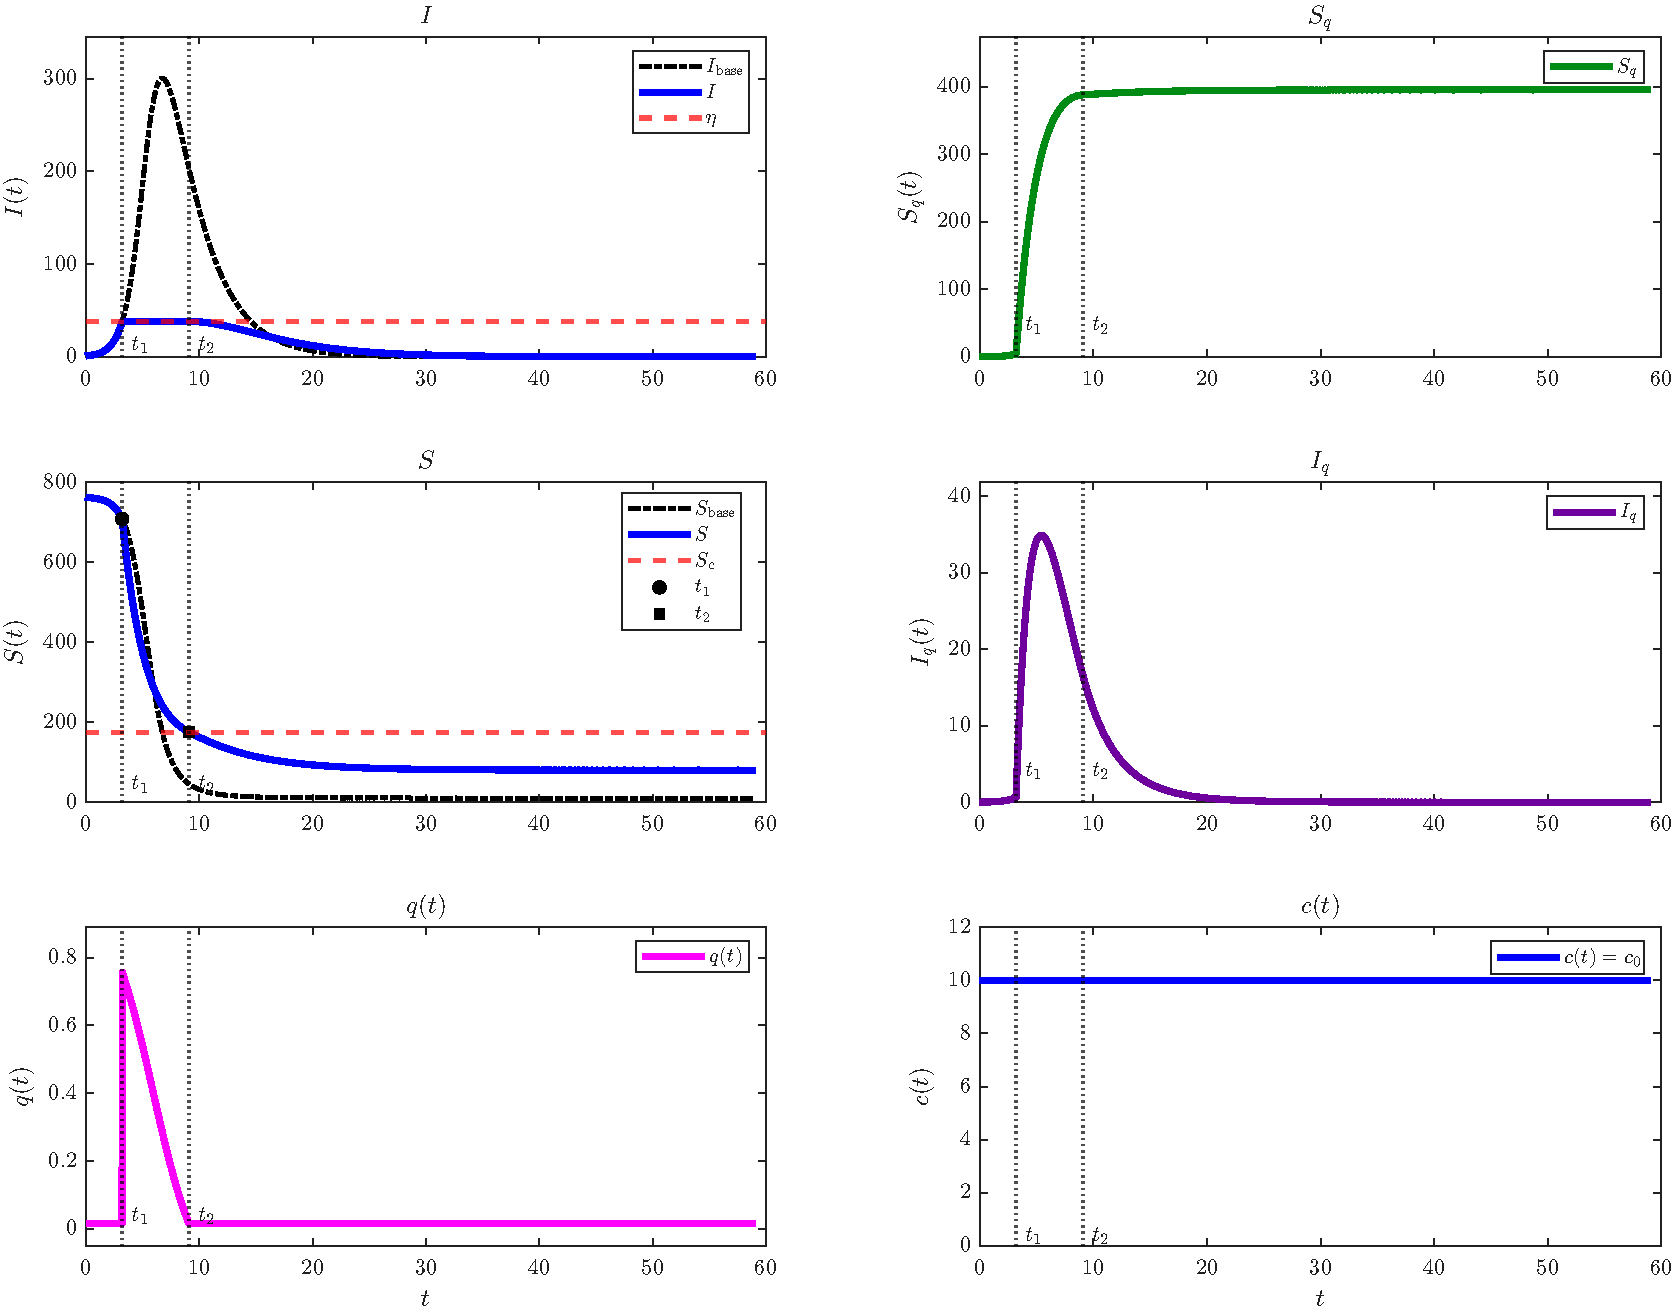
\includegraphics[width=0.7\textwidth]{figures/optimal_control_with_quarantine_panels.pdf}
\caption{仅隔离阈值控制与常规控制的时间轨迹。参数为 $N=763$、$S_0=762$、$I_0=1$、$S_q(0)=I_q(0)=R(0)=0$、$\beta=0.155$、$c_0=10\ \mathrm d^{-1}$、$q_0=0.01526$、$\gamma=\delta_q=0.3504\ \mathrm d^{-1}$、$\eta=0.05N=38.15$。此处的阈值比例用于说明解析结果，不作具体 ICU 容量换算。阈值控制在 $[t_1,t_2]$ 内维持 $I=\eta$，$q_c$ 从启动最大值下降至 $q_0$；$c(t)$ 始终为 $c_0$。横轴为自初始时刻起的天数。}
\label{fig:scenario1:single-sim}
\end{figure}


图\ref{fig:scenario1:single-sim}说明仅隔离策略的完整过程。本节比较常规接触率和感染阈值对多个结果指标的影响，参数取值见各图图注。不同 $c_0$ 对应不同的常规接触水平，每条轨迹内仍保持 $c(t)\equiv c_0$。当 $\eta=0.05N$ 时，控制触发边界为
\[
c_{0,\min}(0.05N)\approx3.3270.
\]
仅在满足触发条件的参数范围内计算控制指标。补充表\ref*{tab:sup:baseline}分别列出固定 $\eta/N=5\%$ 与固定 $c_0=10$ 的结果；控制轨迹见图\ref{fig:baseline:q-joint}，多指标变化见图\ref{fig:scenario1_summary_c0}、\ref{fig:scenario1_summary_eta}。


\begin{figure}[htbp]
\centering
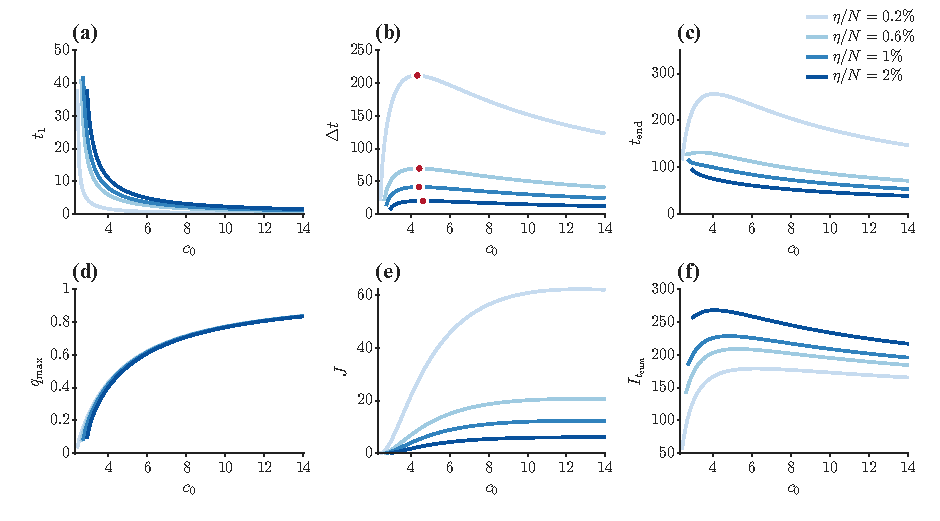
\includegraphics[width=\textwidth]{figures/layout_v5/c0_sensitivity_selected_eta.pdf}
\caption{不同阈值比例下各指标随 $c_0$ 的变化。固定 $N=763,S_0=762,I_0=1,\beta=0.155,\gamma=0.3504\ \mathrm d^{-1},q_0=0.01526$，$\eta/N=0.2\%,0.6\%,1\%,2\%$，红色圆点表示 $\Delta t$ 的数值极大值。}
\label{fig:scenario1_summary_c0}
\end{figure}


\begin{figure}[htbp]
\centering
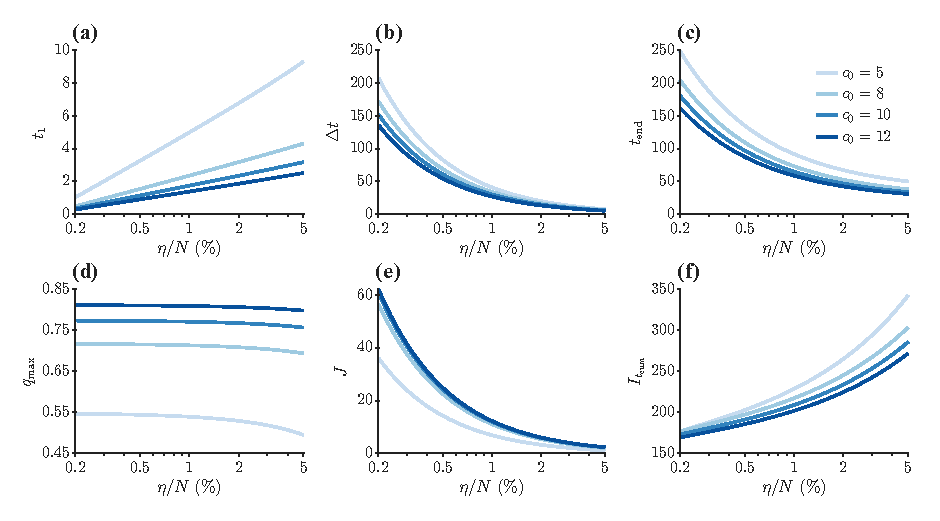
\includegraphics[width=\textwidth]{figures/layout_v5/eta_sensitivity_selected_c0.pdf}
\caption{不同常规接触率下各指标随 $\eta/N$ 的变化。固定 $N=763,S_0=762,I_0=1,\beta=0.155,\gamma=0.3504\ \mathrm d^{-1},q_0=0.01526$，$c_0=5,8,10,12$。}
\label{fig:scenario1_summary_eta}
\end{figure}


%\clearpage

图~\ref{fig:baseline:q-joint}(a) 中，$c_0=4$ 时 $q_{\max}=0.3413<\qinf\approx0.4083$，不存在内部拐点；$c_0=5,8,10,12$ 时均存在唯一内部拐点。图~\ref{fig:baseline:q-joint}(b) 中，各拐点对应的隔离率相同，但启动时间和控制持续时间随阈值改变。

由表~\ref*{tab:sup:baseline} 和图~\ref{fig:scenario1_summary_c0}，增大 $c_0$ 会提高启动点 $S^*$ 和最大隔离率 $q_{\max}$，并使启动时间提前。控制时长在所考察范围内先增加后减小。例如，$\eta/N=5\%$ 时，
\[
\Delta t(3.3470)=2.0432,\qquad
\Delta t(5)=7.5778,\qquad
\Delta t(12)=5.3007\ {\rm d}.
\]
相应的数值极大值位于 $c_0\approx5.1$，约为 $7.5788$ 天。对于 $\eta/N=0.2\%,0.6\%,1\%,2\%$，极大值位置分别约为 $c_0=4.3,4.4,4.4,4.6$，对应时长为 $211.5435,69.8417,41.5169,20.2813$ 天。

表~\ref*{tab:sup:baseline} 和图~\ref{fig:scenario1_summary_eta} 表明，增大 $\eta$ 会推迟控制启动、降低 $q_{\max}$，并缩短阈值控制期。当 $c_0=10$、$\eta/N$ 从 $0.2\%$ 增至 $2\%$ 时，
\[
\Delta t:152.0574\to15.0431,\qquad
t_{\rm end}:180.5821\to46.8029,
\]
\[
J:60.8005\to5.8888,\qquad
\Itcum:173.0314\to233.7810.
\]
在这一参数范围内，提高阈值缩短了阈值控制期和清零时间，降低了控制成本，但增加了累计感染。图~\ref{fig:scenario1_heatmaps_c0_eta} 给出这些指标在 $(\eta/N,c_0)$ 平面上的变化。触发边界 $c_{0,\min}(\eta)$ 随 $\eta$ 增大而升高；其下方的常规感染峰值低于阈值，无需启动加强隔离。

\FloatBarrier
\subsection{两组参数下的四种分配}
\label{sec:joint:compare-numerics}
% BEGIN JOINT_EXTRA:comparison
在同一完整初值、阈值和退出目标下，比较仅减少接触、显式族 $\alpha=0.5$、仅隔离和类内最小二次成本四种分配。基准参数沿用图\ref{fig:scenario1:single-sim}，西安参数沿用第\ref{sec:xian}节的未取整初值；两组均取 $w_c=1,w_q=2$。结果见表\ref{tab:joint:compare}及图\ref{fig:joint:compare}。

基准参数下，类内最小成本为 $J_{\min}\approx2.1183$，控制时长约为 $7.7536$ d；仅隔离的对应值为 $2.2236$ 和 $5.9026$ d。总累计新增感染分别约为 $306.6$ 和 $285.7$ 人。相对仅隔离，成本降低约 $4.7\%$，控制时间增加约 $31.4\%$，总累计新增感染增加约 $7.3\%$。最低成本分配的控制时间更长、累计新增感染更多、控制期新增隔离易感者更少，与式\eqref{eq:joint:cumulative}--\eqref{eq:joint:quarantine}的排序一致。

两组参数下，最低成本分配都分为前后两段。基准和西安参数的启动状态分别为 $S^*/S_c\approx4.044$ 和 $4.378$，均大于 $S_{\rm sw}/S_c\approx2.265$ 和 $2.548$。由命题\ref{prop:joint:global-structure}，任一类内最小成本可测控制在 $S_c<S<S_{\rm sw}$ 上几乎处处同时使用两种措施；$S>S_{\rm sw}$ 时该命题只说明仅隔离是局部最小点。对 $w_c=1,w_q=2$ 比较全部候选后，数值结果显示 $S>S_{\rm sw}$ 上的全局最小点就是仅隔离，切换发生在 $S=S_{\rm sw}$ 处且分配连续；退出时两种控制回到常规水平（权重的影响见第\ref{sec:joint:weights-numerics}节）。基准参数下，仅隔离段约为 $1.61$ d，占控制时长的 $21\%$，但 $S$ 在该段的下降占平台期总下降的 $58\%$；此后接触率最大降低约 $19.8\%$。西安参数下相应为 $25.46$ d、$23\%$、$54\%$ 和 $28.2\%$。平台期成本和控制时长都是关于 $S$ 的积分，两种分配在 $S\ge S_{\rm sw}$ 一段的贡献相同，表\ref{tab:joint:compare}中二者 $J$ 与 $\Delta t$ 的差别只来自 $S_c<S<S_{\rm sw}$ 一段。在这一段，最低成本分配取 $c_c(S)<c_0$，由 $\dot S=-(\eta/N)[c_c(S)S-c_0\bar S]$，相较仅隔离，$S$ 下降较慢，控制时间因而延长；隔离强度相应降低，二次成本减小。

感染人数上限约束的是 $I$，不是 $I+I_q$。在各自 $[0,t_{\rm end}]$ 上，基准参数下仅隔离、最低成本分配与仅减少接触的 $\max(I+I_q)/\eta$ 分别约为 $1.92$、$1.89$ 和 $1.02$；西安参数下相应为 $4.73$、$4.73$ 和 $1.46$。西安参数下，仅隔离与最低成本分配的这一峰值都出现在启动后约 $7.62$ d，此时两者仍处于分配相同的 $S>S_{\rm sw}$ 一段，故峰值相同；基准参数下仅隔离的峰值出现在两者分开之后，最低成本分配的峰值略低。这些是现存感染人数，不是医疗或 ICU 占用；图\ref{fig:joint:compare}(c)中的水平线 $1$ 只作归一化参照。

\begingroup
\begin{table}[htbp]
\centering\small
\setlength{\tabcolsep}{3.5pt}
\renewcommand{\arraystretch}{1.25}
\begin{threeparttable}
\caption{相同阈值与启动、退出要求下四种分配的结果（$w_c=1,w_q=2$）}
\label{tab:joint:compare}
\begin{tabularx}{\linewidth}{@{}>{\raggedright\arraybackslash}Xccccc@{}}
\toprule
分配 & \shortstack{控制时长\\$\Delta t$（d）} & \shortstack{清零时刻\\$t_{\rm end}$（d）} & \shortstack{总累计\\新增感染} & \shortstack{控制期新增\\隔离易感者} & $J$（d）\\
\midrule
\multicolumn{6}{@{}l}{基准参数：$N=763$，$\eta=0.05N$；新增人数单位为人}\\
仅减少接触 & 36.26 & 64.13 & 628.6 & 40.9 & 11.9390\\
显式族 $\alpha=0.5$ & 9.24 & 37.11 & 323.4 & 346.2 & 2.5462\\
仅隔离 & 5.90 & 33.77 & 285.7 & 383.9 & 2.2236\\
类内最小成本 & 7.75 & 35.62 & 306.6 & 363.0 & 2.1183\\
\midrule
\multicolumn{6}{@{}l}{西安参数：$\eta=0.002N$；新增人数单位为 $10^6$ 人}\\
仅减少接触 & 308.79 & 481.83 & 3.8566 & 6.5004 & 109.3648\\
显式族 $\alpha=0.5$ & 124.57 & 297.60 & 2.6390 & 7.7180 & 44.5286\\
仅隔离 & 85.07 & 258.10 & 2.3779 & 7.9791 & 40.7686\\
类内最小成本 & 108.81 & 281.84 & 2.5348 & 7.8222 & 38.0209\\
\bottomrule
\end{tabularx}
\begin{tablenotes}[flushleft]\footnotesize
\item 注：每组沿用同一完整初值、首次上升至 $I=\eta$ 的启动规则和 $S=S_c$ 的退出目标，各自恢复常规后在 $I$ 下降至 $1$ 时终止。累计新增感染不包含初始感染者；新增隔离易感者只统计控制期。$J$ 为式\eqref{eq:cost:J}的二次成本，不由线性 $J_c,J_q$ 加总。西安参数及未取整初值见第\ref{sec:xian}节；表内单位和显示精度按行组区分。
\end{tablenotes}
\end{threeparttable}
\end{table}
\endgroup
% END JOINT_EXTRA:comparison

在同一全市人口、未取整拟合初值及 $\eta=0.002N$ 下，第\ref{sec:joint:compare-numerics}节又比较了四种阈值分配（表\ref{tab:joint:compare}）。类内最小成本从仅隔离的 $40.7686$ 降至 $38.0209$，控制时长由 $85.07$ 延长至 $108.81$ d，总累计新增感染由约 $2.3779\times10^6$ 增至 $2.5348\times10^6$。相对变化分别约为成本 $-6.7\%$、控制时长 $+27.9\%$、总累计新增感染 $+6.6\%$。因此，这里的成本降低不伴随感染指标同时改善。
\begin{figure}[htbp]
\centering
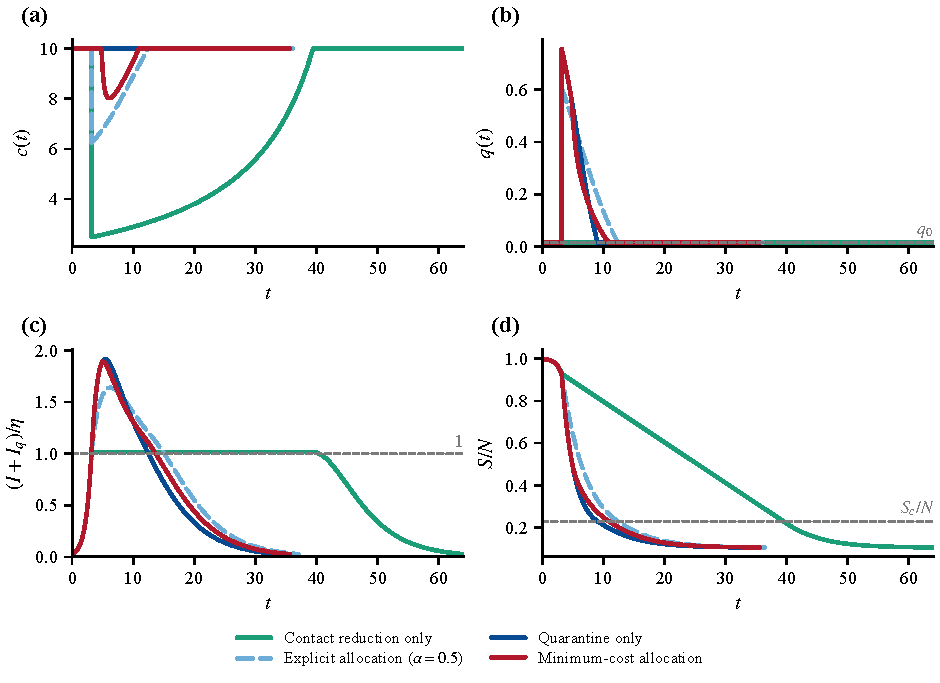
\includegraphics[width=\textwidth]{figures/joint_v2/joint_compare_baseline.pdf}
\caption{基准参数下相同启动与退出要求的四种分配（$N=763$，$\eta=0.05N$，$w_c=1,w_q=2$）。(a) 接触率；(b) 隔离率；(c) 现存感染人数与阈值之比 $(I+I_q)/\eta$；(d) 社区易感者比例。各轨迹画至自身的动态清零时刻，横轴 $t$ 为自共同初始时刻起的天数。控制跳变按分段数据绘制；(c) 的水平 $1$ 为归一化参照，不是本文对总感染现患人数的约束。}
\label{fig:joint:compare}
\end{figure}

\FloatBarrier
% TODO（阶段4e-3）：迁入的西安数值段与本节表格仍有重复，按批准范围精简。
\subsection{能力限制下的可行性与受限分配}
\label{sec:joint:capacity-numerics}
% BEGIN JOINT_EXTRA:capacity
\def\jointcapacitypostexitdays{1}
图\ref{fig:joint:capacity}将能力平面分成至少一种单控制可行、两种单控制均不可行但联合可行、规定触发状态下不可行三个区域。仅隔离可行要求 $q_{\rm cap}\ge q_{\max}$，仅减少接触可行要求 $c_{\min}\le c_0S_c/S^*$；二者均不成立时由式\eqref{eq:joint:feasibility}判断联合可行性，边界等号归入可行侧。灰色区域的不可行只针对在 $I$ 首次达到 $\eta$ 时启动、在 $S=S_c$ 退出的平台控制。

基准参数代表点取 $c_{\min}/c_0=0.5$、$q_{\rm cap}=0.6$。仅隔离需要 $q_{\max}\approx0.756$，仅减少接触需要把接触率降低约 $75.3\%$，两者均超出能力限制，联合控制可行。受限类内最小成本约为 $2.3611$，控制时长约为 $8.34$ d，比无额外能力限制时分别增加约 $11.5\%$ 和 $7.5\%$。西安代表点取 $c_{\min}/c_0=0.5$、$q_{\rm cap}=0.75$，相应为 $41.6166$ 和 $116.75$ d，增幅约为 $9.5\%$ 和 $7.3\%$。

图\ref{fig:joint:capacity}(c)给出基准代表点的时间控制。启动后约 $1.94$ d 内，隔离比例停在上限 $0.6$，接触率同时降低，降幅由启动时的约 $39.1\%$ 随 $S$ 下降而减小；$S$ 降至 $(1-q_0)S_c/(1-q_{\rm cap})\approx2.462S_c$ 时，仅隔离已能维持平台，接触率回到 $c_0$。随后经过约 $0.26$ d 的仅隔离段，$S<S_{\rm sw}$ 后两种措施同时使用直至退出。在 $S\le(1-q_0)S_c/(1-q_{\rm cap})$ 上，无额外限制时的逐状态最小点满足两项能力限制，因而也是受限问题的逐状态最小点，数值核查显示同一 $S$ 处两者的 $c_c(S)$、$q_c(S)$ 相同。这里的一致只指同一易感者状态下的控制：受限分配到达同一 $S$ 的时刻较晚，$I_q$、$S_q$ 等状态也不同，并非相同时刻的完整轨迹相同。由于 $J$ 与 $\Delta t$ 都是关于 $S$ 的积分，能力限制只改变启动后的前一段分配，二者的增加都来自这一段。西安代表点的结构相同，隔离比例停在上限约 $30.38$ d。有能力限制时，可达到的最短和最长控制时长由实际允许区间的上下界给出，不再对应两种单控制。
% END JOINT_EXTRA:capacity

\begin{figure}[htbp]
\centering
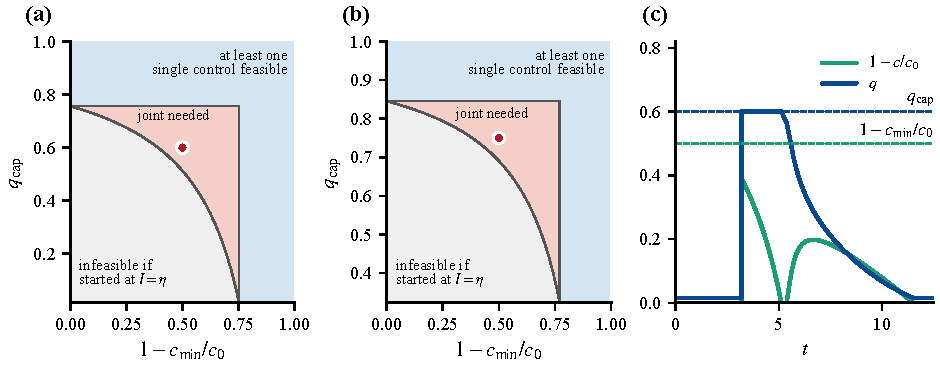
\includegraphics[width=\textwidth]{figures/joint_v2/joint_capacity.pdf}
\caption{能力限制下的可行区域与代表轨迹。(a) 基准参数；(b) 西安参数。横轴为最大接触减少比例 $1-c_{\min}/c_0$，纵轴为隔离比例上限 $q_{\rm cap}$；灰色、浅红色、浅蓝色分别表示规定触发状态下不可行、需联合控制、至少一种单控制可行，边界归入可行侧。红点为代表能力组合。(c) 基准代表点的受限最低二次成本分配，绘至名义退出后\jointcapacitypostexitdays{}天，横轴 $t$ 的单位为天。}
\label{fig:joint:capacity}
\end{figure}

\FloatBarrier
\subsection{成本权重与分配结构}
\label{sec:joint:weights-numerics}
% BEGIN JOINT_EXTRA:phase
为比较分配结构，固定 $w_c=1$ 并改变 $r=w_q/w_c$；其余参数及状态固定时，权重对逐状态最小点的影响仅通过比值 $r$。图\ref{fig:joint:phase}给出 $r\in[0.1,20]$ 上 $161$ 个对数等距取值的结果，颜色 $y=(1-c_c^*/c_0)/(1-S_c/S)$ 是接触减少相对于仅减少接触端点的比例，$y=0$ 与 $y=1$ 分别对应两种单控制（隔离强度不是 $1-y$）。全局切换点由端点与内部驻点的成本比较确定；命题\ref{prop:joint:global-structure}中的 $S_{\rm sw}$ 只给出端点的局部性质，基准和西安参数分别约为 $2.265S_c$ 和 $2.548S_c$。

在所计算的 $161$ 个网格点上，基准参数直到网格点 $r\approx3.13$、西安参数直到网格点 $r\approx2.65$，各点的全局切换点都与 $S_{\rm sw}$ 重合且分配连续：$S>S_{\rm sw}$ 时取仅隔离，$S<S_{\rm sw}$ 时两种措施同时使用。默认 $r=2$ 不是网格点；第\ref{sec:joint:compare-numerics}节在 $r=2$ 下单独完成的候选比较同样给出 $S=S_{\rm sw}$ 处的连续切换。从相邻的网格点 $r\approx3.24$（基准）和 $r\approx2.74$（西安）起，仅隔离段在 $S$ 降至 $S_{\rm sw}$ 之前结束：$S$ 略大于 $S_{\rm sw}$ 时仅隔离仍是局部最小点，但内部的另一局部最小点成本更低。在其后的网格点上，切换点随 $r$ 增大移向启动状态，接触率在切换处由 $c_0$ 跳到内部值；例如 $r\approx4.98$ 时，基准和西安的切换点约为 $2.544S_c$ 和 $3.367S_c$，接触率分别跳至约 $0.539c_0$ 和 $0.369c_0$。出现仅隔离段的最大网格点为 $r\approx13.00$（基准）和 $7.41$（西安），从 $r\approx13.44$ 和 $7.66$ 起，整个平台期不再出现仅隔离段。相邻网格点显示了上述两处结构变化，但未进一步确定连续权重下的精确转折位置或证明其唯一性。靠近退出时，各 $r$ 下的 $y$ 趋于 $r/(1+r)$，与命题\ref{prop:joint:terminal-allocation}一致。改变 $r$ 即改变成本标准，不同 $r$ 下的 $J$ 不直接比较。
% END JOINT_EXTRA:phase

\begin{figure}[htbp]
\centering
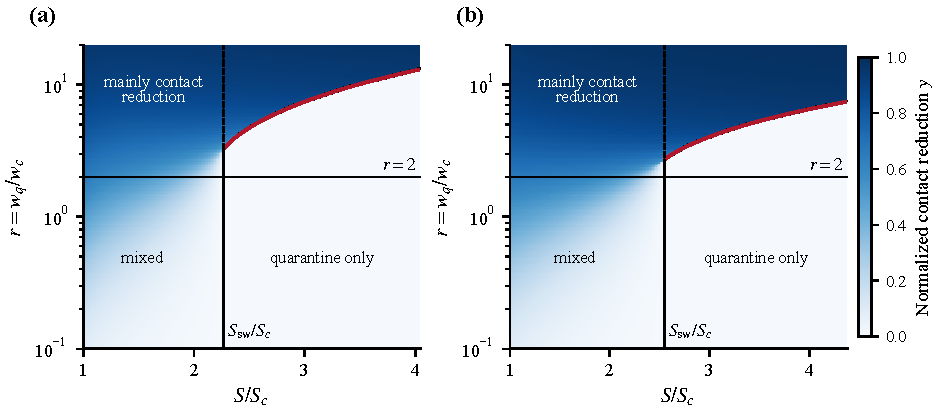
\includegraphics[width=\textwidth]{figures/joint_v2/joint_phase_weights.pdf}
\caption{固定 $w_c=1$、改变 $r=w_q/w_c$ 时的类内最低二次成本分配。(a) 基准参数；(b) 西安参数。颜色为 $y=(1-c_c^*/c_0)/(1-S_c/S)$，$y=0$ 为仅隔离，$y=1$ 为仅减少接触。竖直线位于局部阈值 $S_{\rm sw}/S_c$，其实线段与红色曲线为数值比较得到的全局切换边界，红色曲线处接触率跳变；水平点线为默认 $r=2$。沿控制时间，$S$ 从右向左减小。}
\label{fig:joint:phase}
\end{figure}

\FloatBarrier
% BEGIN JOINT_EXTRA:duration
\subsection{成本—控制时长关系}
\label{sec:joint:duration-numerics}
图\ref{fig:joint:frontier}给出基准参数下 $470$ 个经数值核查的乘子解，每个解报告实际 $\Delta t$ 与原二次成本 $J$。注记\ref{rem:joint:duration-constraint}给出的是充分条件：取得时长匹配的乘子解 $c_\kappa$ 时，它是约束 $\Delta t=\Delta t[c_\kappa]$ 下的类内最小成本控制。两种单控制之间的每个时长都可由允许控制实现，但计算点之间的时长未逐一取得匹配乘子，这些时长上的最低成本未由此确定。

在当前参数下，计算点显示最低成本附近 $J$ 对 $\Delta t$ 不敏感。若要求 $\Delta t\le T$ 且 $\Delta t[c_0]\le T\le\Delta t[c_c^*]$，仅隔离满足这一限制，故成本下界为无额外时长限制的最低二次成本 $J_{\min}=J[c_c^*]$，上界为仅隔离的实际二次成本 $J[c_0]$。两个时长端点约为 $5.90$ 和 $7.75$ d，而 $J[c_0]\approx1.05J_{\min}$ 仅作显示近似；$\kappa\ge0$ 的计算点均落在上述实际成本范围内。$\kappa<0$ 一侧，满足 $J\le1.10J_{\min}$ 的计算点中最大时长约为 $11.09$ d，下一个计算点（$11.40$ d）约为 $1.12J_{\min}$；$11.09$ d 不是精确的临界时长。仅减少接触端点（$36.26$ d）的 $J$ 约为 $5.64J_{\min}$。$\kappa<0$ 的解对应时长下限，由式\eqref{eq:joint:quarantine}等价于限制控制期新增隔离易感者人数；若只考虑 $J$ 与 $\Delta t$，这些解的两项都大于最低成本点，因此整条曲线不是同时最小化二者的效率前沿。显式 $\alpha$ 族属于同一允许控制类，只作对照。

\begin{figure}[htbp]
\centering
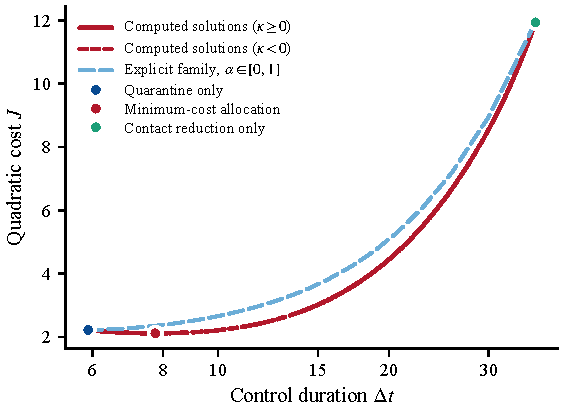
\includegraphics[width=0.6\textwidth]{figures/joint_v2/joint_frontier_baseline.pdf}
\caption{基准参数下二次成本与控制持续时间的关系。红色曲线连接已核查的 $J+\kappa\Delta t$ 最小化解，实线与短虚线分别对应 $\kappa\ge0$ 和 $\kappa<0$；连线不表示中间时长已有匹配乘子。浅蓝虚线为显式 $\alpha$ 族，圆点为两种单控制与无时长限制的最低成本分配。横轴为对数坐标，$\Delta t$ 与 $J$ 的单位均为天。}
\label{fig:joint:frontier}
\end{figure}
% END JOINT_EXTRA:duration

\FloatBarrier


% ===== 08_xian =====
\section{西安参数下的情景比较与退出代价}
\label{sec:xian}

本节先采用 He、Tang 和 Xiao~\cite{He2023TDINN} 给出的西安疫情 TDINN 控制函数和日报数据，将 $c(t)\equiv c_0$ 的仅隔离控制用于西安参数下的数值计算，并与 TDINN 重构控制及常规控制比较。同一起止状态下的联合阈值分配另见第\ref{sec:joint:compare-numerics}节和表\ref{tab:joint:compare}，并在本节简述其结果。TDINN 控制同时降低接触率、提高隔离比例；这里的仅隔离控制对照则保持接触率不变，仅通过提高隔离比例使社区感染者人数 $I(t)$ 不超过 $\eta$。记社区感染者 $I(t)$、新增社区感染 $I_{\rm new}(t)$、新增隔离感染 $I_{q_{\rm new}}(t)$、社区累计新增感染 $I_{\rm cum}(t)$、隔离累计新增感染 $I_{q_{\rm cum}}(t)$，以及总累计新增感染 $\Itcum(t)=I_{\rm cum}(t)+I_{q_{\rm cum}}(t)$。

% TODO（阶段4f）：章首路线图及“后续/下一节”指向按新结构改写。
\subsection{数据、重构参数与初值}
病例数据包含社区发现病例数 $I_{\rm new}(t)$ 和隔离发现病例数 $I_{q_{\rm new}}(t)$，覆盖 2021 年 12 月 9 日至 2022 年 1 月 17 日共 40 天，其中社区发现 583 例、隔离发现 1467 例，合计 2050 例（图~\ref{fig:xian:observed-fit}）。TDINN 控制曲线取自文献~\cite{He2023TDINN} 表 3 中西安的拟合结果 $c_2(t),q_2(t)$：
\begin{equation}
c_{\rm TDINN}(t)=(12.8872-3.4625)e^{-(0.0463t)^2}+3.4625,\qquad
q_{\rm TDINN}(t)=(0.3230-0.9844)e^{-(0.0452t)^2}+0.9844,
\end{equation}
因此常规初始控制水平为 $c_0=12.8872,\ q_0=0.3230$。


在系统~\eqref{eq:model:full} 中，引入累计变量 $I_{\rm cum}(t),I_{q_{\rm cum}}(t)$，满足
\begin{equation}
\dot I_{\rm cum}(t)=\frac{\beta c(t)(1-q(t))S(t)I(t)}{N},\qquad
\dot I_{q_{\rm cum}}(t)=\frac{\beta c(t)q(t)S(t)I(t)}{N}.
\end{equation}
总人口取西安市 2021 年末常住人口 $N=13{,}163{,}000$；传播参数固定为文献~\cite{He2023TDINN} 表 1 的估计值 $\beta=0.1498,\ \gamma=0.2953,\ \delta_q=0.3531$。由于原文未给出拟合初值，本文设 $R(0)=0$，从而 $N=S_0+I_0$，只用最小二乘估计 $I_0$ 并令 $S_0=N-I_0$；拟合准则为每日新增 $I_{\rm new},I_{q_{\rm new}}$ 与累计 $I_{\rm cum},I_{q_{\rm cum}}$ 四项均方误差之和。拟合结果见表~\ref{tab:xian_initial_fit}。

拟合得到的 $I_0$ 是给定时间原点和控制函数下的模型初值，不对应整数病例数。若改取 $I_0=1$，模型计算的 $40$ 天累计病例约为 $1.08\times10^6$，远高于观测值，见表~\ref*{tab:sup:initial}。


\begin{figure}[htbp]
\centering
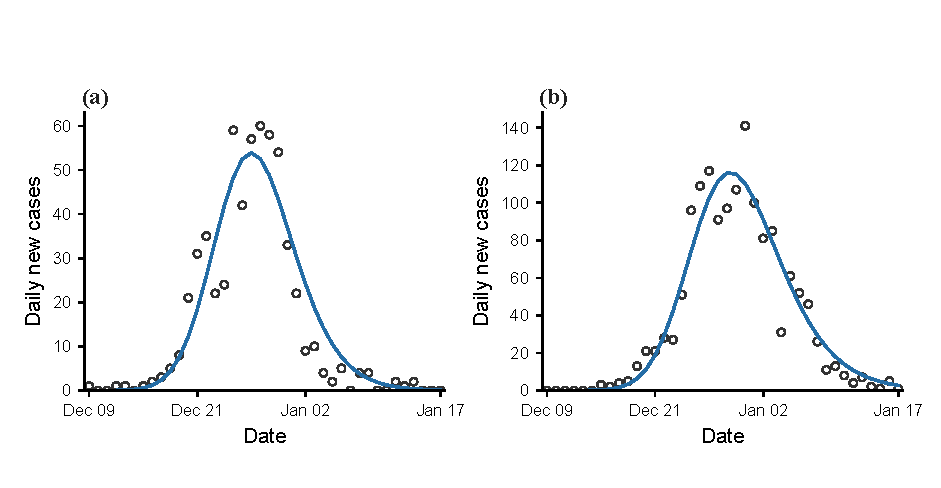
\includegraphics[width=\textwidth]{figures/layout_v5/xian_observed_fit.pdf}
\caption{西安疫情观测窗口内的日新增病例与 TDINN 重构。(a) 社区发现病例；(b) 隔离发现病例。点为观测值，实线取自三策略比较所用的同一 TDINN 轨迹，以相邻整数日累计量之差计算日新增。40 个日区间从 2021 年 12 月 9 日起算；本图用于拟合重构的比较，并非独立数据验证。}
\label{fig:xian:observed-fit}
\end{figure}

参数与初始条件列于第\ref{sec:num:methods}节的表\ref{tab:xian_initial_fit}。
\subsection{外部参照}
三类策略均计算至各自的清零时间，即 $I(t)$ 超过 $1$ 后再次下降至 $1$ 的时刻。成本采用第~\ref{sec:cost}~节的定义，权重为 $w_c=1,w_q=2$：TDINN 从初始时刻积分至清零，阈值控制仅在 $[t_1,t_2]$ 内产生额外成本，常规控制的额外成本为零。

图\ref{fig:xian:strategy-process}给出三类策略下的感染、总累计新增感染、有效再生数与控制轨迹，主要指标列于表\ref{tab:xian_summary}。

\begin{figure}[htbp]
\centering
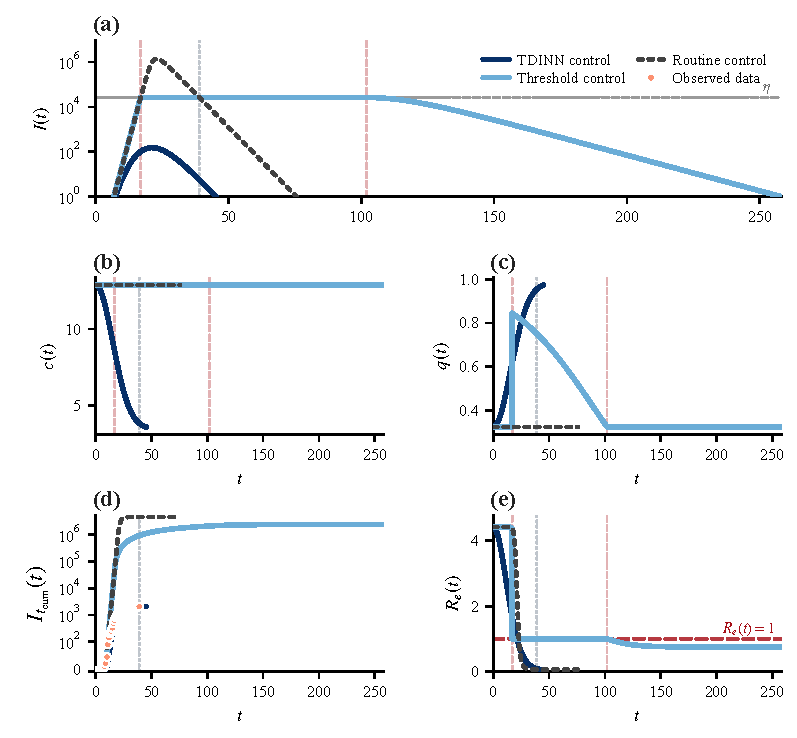
\includegraphics[width=135mm]{figures/layout_v5/xian_strategy_process.pdf}
\caption{$\eta=0.002N$ 时三策略的全过程比较。(a) 社区感染者人数 $I(t)$；(b) 接触率 $c(t)$；(c) 隔离比例 $q(t)$；(d) 总累计新增感染 $\Itcum(t)$；(e) 有效再生数 $R_e(t)$。各轨迹分别画至自身的清零时间，横轴使用同一时间原点，$t$ 的单位为天。(a) 为对数纵轴；(d) 为对称对数纵轴（线性区阈值为 $100$ 人），散点为观测累计量；(e) 的水平虚线为 $R_e=1$。浅红色竖虚线标记控制启动与解除，灰色竖点线标记观测窗口结束。}
\label{fig:xian:strategy-process}
\end{figure}

\begin{table}[htbp]
\centering\small
\setlength{\tabcolsep}{3.5pt}
\renewcommand{\arraystretch}{1.25}
\begin{threeparttable}
\caption{西安参数下三种策略的感染结局与干预指标}
\label{tab:xian_summary}
\begin{tabular*}{\linewidth}{@{\extracolsep{\fill}}lS[table-format=7.0]S[table-format=7.0]S[table-format=3.2]S[table-format=2.4]@{}}
\toprule
策略 & {\shortstack{社区感染峰值\\（人）}} & {\shortstack{总累计新增感染\\（人）}} & {\shortstack{清零时间\\（d）}} & {$J$（d）}\\
\midrule
TDINN 控制 & 153 & 2106 & 45.29 & 49.3894\\
仅隔离控制 & 26326 & 2377943 & 258.10 & 40.7686\\
常规控制 & 1377552 & 4587183 & 75.57 & 0.0000\\
\bottomrule
\end{tabular*}
\begin{tablenotes}[flushleft]\footnotesize
\item 注：$\eta=0.002N$ 为设计情景；各策略沿用原文规定的社区清零终点；人数四舍五入至整数。用于后续比较的 TDINN 参照为峰值152.55、总累计2105.63、清零时间45.29 d、$J=49.39$。$J$ 为二次加权积分，不由线性指标 $J_c,J_q$ 直接加总。阈值策略的启动、解除与控制时长分别为 $16.90$、$101.97$、$85.07$ d。
\end{tablenotes}
\end{threeparttable}
\end{table}


采用全市人口及 $\eta=0.002N$ 时，阈值控制将社区感染峰值限制为 $26{,}326$，阈值控制持续约 $85.07$ 天，清零时间约为 $258.10$ 天，总累计新增感染约为 $2.38\times10^6$。TDINN 重构的峰值和累计新增感染分别约为 $153$ 和 $2106$。阈值控制的二次加权成本为 $40.77$，低于 TDINN 的 $49.39$，但感染峰值、累计新增感染和清零时间均较大。后文采用更精确的 TDINN 参照值 $I_{\rm peak}^{\rm T}=152.55$、$\Itcum^{\rm T}=2105.63$ 和 $J^{\rm T}=49.39$。

有效再生数为 $R_e(t)=\beta c(t)(1-q(t))S(t)/(\gamma N)$。常规控制下 $R_e(0)\approx4.43$，感染人数初期快速增长；TDINN 同时降低接触率并提高隔离比例，使 $R_e$ 较快降至 $1$ 以下；阈值控制则在阈值控制期保持 $R_e=1$，待 $S$ 下降至 $S_c$ 后恢复常规隔离比例，感染人数才开始下降。因此，较低的加权成本在这里伴随着更长的感染持续时间和更高的累计新增感染。

TDINN 仍为另一终止任务下的外部参照，不属于固定启动状态、在同一阈值上维持恒定感染的要求和退出状态的四策略比较类，也不据此宣称它已被联合阈值策略支配。

\subsection{低阈值与常规退出要求的代价}
\label{sec:xian:threshold-scale}
本节采用西安人口及拟合传播参数，取代表性社区感染上限
\begin{equation}
\eta=0.002N=26{,}326.
\end{equation}
该阈值为设计情景，其医疗资源相关的量级参考见补充材料第\ref{sec:sup:threshold-scale}节。各策略采用同一阈值比较，阈值变化的影响由后续敏感性分析考察。
按第~\ref{sec:s1}节，常规控制下临界易感人数 $S_c=\gamma N/[\beta c_0(1-q_0)]=2{,}974{,}125.41$；数值求得达到阈值时刻 $t_1=16.90$、启动点 $S^*=13{,}020{,}440.75$。阈值控制期由理论开环控制 $q_c(t)=1-\gamma N/[\beta c_0 S(t)]$（其中 $S(t)=\bar S+(S^*-\bar S)e^{-c_0\eta(t-t_1)/N}$，$\bar S=\gamma N(1-\beta)/(\beta c_0)$）维持 $I(t)\equiv\eta$，解除时刻
\[
t_2=t_1+\frac{N}{c_0\eta}\ln\frac{S^*-\bar S}{S_c-\bar S}\approx101.97,
\]
控制时长约 $85.07$ 天；启动隔离比例 $q_c(t_1)=0.8454$，终点 $q_c(t_2)=q_0=0.3230$。阈值控制阶段最大数值偏差约为 $1.35\times10^{-6}$。

\[
\eta\downarrow\ \Rightarrow\ t_1\downarrow,\qquad \Delta t\uparrow,\qquad J\uparrow,\qquad t_{\rm end}\uparrow.
\]
当 $\eta/N$ 从 $0.01$ 降至 $0.0001$ 时，启动时间仅由 $18.55$ 天提前至 $13.92$ 天，控制时长却由 $16.61$ 天增加至 $1710.66$ 天，清零时间达到 $2209.55$ 天。降低阈值减慢了阈值控制期的易感者减少过程，其对控制时长的影响远大于对启动时间的影响。


在西安全市人口设定（$N=13\,163\,000$，$c_0=12.8872$）下，由控制时长闭式
\[
\Delta t=\frac{N}{c_0\eta}\ln\frac{S^{*}-\bar S}{S_c-\bar S}
\]
有$\eta=0.002N=26326$ 时 $\Delta t\approx85$ 天；$\eta=152.55$ 时，$S^{*}\approx1.3162\times10^{7}$、对数因子约为 $2.205$，从而
\[
\Delta t(\eta=152.55)\approx1.48\times10^{4}\ \text{d}\approx 40.5\ \text{年}.
\]
规定退出状态也限制了累计新增感染。将本节参数代入命题\ref{prop:exit-infection-lower-bound}，得
\[
\Itcum(t_2)\ge\beta(S_0-S_c)\approx1.53\times10^6.
\]
因此，在本节全市人口及传播参数下，任何达到 $S=S_c$ 的策略都不能同时达到约 $2106$ 的累计新增感染参照。联合分配可能降低阈值控制类内的强度成本，但不能解除这个由退出目标造成的感染下界；这个结论也不排除提前消除传播或采用其他退出目标的策略。

这一时长是模型在固定参数和全市人口假设下的外推结果。由时间尺度 $N/(c_0\eta)$ 可见，较大的易感人群和较低的感染阈值会延长阈值控制期。在观测期累计病例约为 $2050$ 的拟合中，$S(t)\approx N$；但阈值策略需要持续至 $S=S_c$，因此其时间估计对人口规模尤为敏感。下一节考察不同有效混合人口下的结果。

完整阈值与接触率扫描见补充材料第\ref{sec:sup:xian}节。
\subsection{有效人口的条件性解释}
\label{sec:dominance}
\label{sec:dom:region}
西安此次疫情的有效混合人口 $N_{\rm eff}$ 未知。本节沿用第~\ref{sec:xian}~节的参数，改变 $N_{\rm eff}$，考察阈值控制满足 TDINN 峰值、成本及时间参照值的参数范围。TDINN 参照固定在全市人口下的拟合结果，阈值控制和常规控制则在各个人口假设下分别计算。本节仍将感染阈值作为设计参数。

数值计算在各人口情景下沿用全市人口下拟合得到的同一个绝对初值 $I_0=1.00659\times10^{-3}$，并取 $S_0=N-I_0$，故 $i_0=I_0/N$ 与 $s_0=1-i_0$ 随人口规模改变。这是本节采用的情景比较约定；若在不同人口下重新拟合，所得初值未必相同。第\ref{sec:scaling-theory}节的规模不变性以固定归一化初值为前提，两者需加以区分。

对于所采用的西安重构轨迹，社区累计新增感染和隔离累计新增感染还给出一个人口相容的必要条件。
\begin{proposition}
\label{prop:dom:floor}
在 $S_q(0)=0$ 的无回流模型中，能够容纳给定重构轨迹的有效人口须满足
\begin{equation}
N_{\rm eff}\ge N_{\rm floor}:=
 I_{\rm cum}^{\rm T}+\frac{I_{q_{\rm cum}}^{\rm T}}{\beta}.
\label{eq:dom:Nfloor}
\end{equation}
\end{proposition}
\begin{proof}
由式\eqref{eq:count-identities}，隔离易感者人数为
$S_q(T)=(1-\beta)I_{q_{\rm cum}}(T)/\beta$。易感者流出的三部分为社区感染、隔离感染和未感染者隔离，故
\[
S_0-S(T)=I_{\rm cum}(T)+I_{q_{\rm cum}}(T)+S_q(T)
=I_{\rm cum}(T)+\frac{I_{q_{\rm cum}}(T)}\beta.
\]
再用 $S_0\le N_{\rm eff}$ 即得。
\end{proof}
当前参照量给出
\[
N_{\rm floor}=607.96+\frac{1497.67}{0.1498}
=1.0606\times10^4\approx1.06\times10^4.
\]
仅计累计新增感染时参照总数为 $2105.63$；计入隔离未感染者后，下界约为该值的 $5.04$ 倍。接近 $N_{\rm floor}$ 意味着大部分初始易感者离开 $S$ 仓室，而不是全部人都被感染。该下界不估计真实有效人口，也不能证明候选人口能够重现全市拟合。

完整比较条件、人口扫描及案例见补充材料第\ref{sec:sup:population}节。

% ===== 10_discussion =====
\section{讨论与结论}
\label{sec:discussion}
\subsection{主要发现与相关研究}
同一社区非隔离感染人数上限下，接触减少与追踪隔离的分配会改变控制时长、累计新增感染和未感染者隔离数量。维持 $I=\eta$ 只约束乘积 $c(1-q)$，而追踪隔离还将未感染接触者移出社区。在固定二维进入状态 $(S^*,\eta)$ 和退出状态 $(S_c,\eta)$ 下，较大的 $c_c(S)$ 配合较高的隔离比例，使 $S$ 下降更快。由定理\ref{thm:joint:comparison}，当 $0<\beta<1$ 时，控制期累计新增感染随控制时长增加，新增隔离易感者人数则减少。因此，无额外能力限制时，仅隔离控制最快且控制期累计新增感染最少，代价是最多未感染者进入隔离。

能力界决定能否完成这一过程，以及每个状态上的允许分配区间。整段可行时，最大允许接触率 $\overline c(S)$ 给出最短控制时长，并在 $0<\beta<1$ 时给出最少的控制期累计新增感染。二次成本则在允许区间内同时权衡干预强度与时间消耗，权重改变其中的成本选择。命题\ref{prop:joint:terminal-allocation}表明，无额外能力限制，或整段可行且 $c_{\min}<c_0$、$q_{\rm cap}>q_0$ 时，最小成本分配在退出附近共同使用两种措施。与某一种单控制的严格成本比较还要求该单控制整段可行。

表\ref{tab:joint:compare}的两组同条件比较显示，最小成本分配相对仅隔离控制降低了 $J$，同时延长控制期并增加累计新增感染。共同完整初值、首次触发规则、阈值 $\eta>1$ 和前后常规控制使控制期感染排序延伸到各自的清零终点，见推论\ref{cor:joint:whole-epidemic}。有限能力代表点和权重网格展示了允许区间与成本选择的不同作用，数值切换仍由全部候选的成本比较确定。局部端点判据、有限权重网格和离散乘子点分别保留第\ref{sec:joint:cost}、\ref{sec:joint:weights-numerics}、\ref{sec:joint:duration-numerics}节的适用范围。

已有研究分别提供了恒定感染策略、分段干预解析和数据重构参照。Miclo 等\cite{Miclo2022ICU}在 SIR 模型、ICU 上限和特定线性成本下得到包含恒定感染阶段的解析最优策略。Zhou 等\cite{Zhou2024SPCI}以分段常数接触率和隔离比例研究干预时机，并用首次积分连接不同阶段。He 等\cite{He2023TDINN}从疫情数据重构随时间变化的接触率和隔离比例，为西安情景提供外部参照。本文在已定义的阈值控制类中，以状态参数化比较两种措施的全部允许分配，分别评价感染流入、未感染者隔离和二次强度成本。

退出要求也决定可达到的感染结局。命题\ref{prop:exit-infection-lower-bound}给出从初始时刻到有限时刻达到 $S=S_c$ 所需的累计新增感染下界，重新分配两种干预不能消除这一限制。对于仅隔离控制，降低阈值使感染峰值更低，却延长维持阈值直至同一易感者水平 $S=S_c$ 的过程。西安外部参照中，仅隔离控制的二次成本低于 TDINN 重构，感染峰值、累计新增感染和清零时间均较高，见表\ref{tab:xian_summary}。两者的阈值与退出要求不同，因而较低的 $J$ 只表示所定义归一化成本较低，不能代替对感染规模和终止任务的评价。

在当前无回流模型中，阈值控制于 $S=S_c$ 恢复常规，随后社区感染人数继续下降。按 $I=1$ 停止积分则给出操作性清零终点，恢复常规后的增长方向仍由该时刻的易感者状态决定。在西安 TDINN 重构的这一终点，若直接恢复常规接触率和隔离比例，状态回代给出 $\beta c_0(1-q_0)S/(\gamma N)\approx4.42>1$。该值是名义参数下的终点状态检查，未模拟后续反弹轨迹。本文保留其原有清零参照，并将其与达到规定退出状态的任务分别解释。

\subsection{适用范围}
\label{sec:dom:limits}
有效人口影响达到退出状态所需减少的易感者规模，但第\ref{sec:dominance}节的人口情景沿用全市拟合的传播参数与绝对初值，未对不同人口重新拟合。接近人口必要下界 $N_{\rm floor}$ 时，$S/N$ 对 $1$ 的偏离增大，原有 $S/N\approx1$ 条件下估计的参数能否移植需要另行判断。实际干预还可能改变混合范围，阈值控制与 TDINN 未必对应同一个有效人口。真实 $N_{\rm eff}$ 需由接触调查、出行信息或防控单元等外部资料确定，相对于固定全市参照的人口情景只能作条件性解释。

初值的缩放方式还影响启动和清零时间。既有近似 $t_1\approx r^{-1}\ln(\theta/i_0)$，其中 $r=\beta c_0(1-q_0)-\gamma$，说明小初值对启动时刻的影响。固定绝对初值时，归一化初值随人口改变；固定归一化初值的规模结论不能替代这一比较。清零终点采用绝对人数 $I=1$，因此时间指标仍含人口尺度。已有初值设定比较中，清零时间边界比成本、控制时长和累计新增感染边界更敏感。在所考察的两种初值设定及数值范围内，未找到同时满足人口相容下界与清零时间参照的参数点；连续允许人口集合仍未确定。完整人口比较的条件与有限证据见补充材料第\ref{sec:sup:population}节。

\FloatBarrier

追踪隔离缩短控制期的机制依赖于隔离易感者不返回社区。允许 $S_q$ 回到 $S$ 后，社区易感者可能不再单调下降，恢复常规后的传播还受回流影响。因此，以 $S$ 参数化控制、由时长确定感染排序及在 $S=S_c$ 退出的后续分析，都需在回流模型中重新建立。西安低阈值情景的长时结果沿用固定参数和无回流假设，适合作为解析基准，其时间估计不能直接解释为实际长期政策效果。

预先生成的时间开环控制依据名义模型维持 $I=\eta$，数值积分验证的是同一模型下的实现。观测误差会影响首次触发的判断，参数失配或执行延迟会使实际感染流入与移出偏离平衡，开环函数本身没有对偏离进行纠正的机制。本文未建立这些误差下的稳定性或峰值保证，提前干预与安全余量需另行评价。监测资料还需估计非隔离感染人数这一存量，某日新增确诊数不能直接替代 $I$。当前能力界限制控制强度，未限制调整速度。

二次成本\eqref{eq:cost:J}计量相对于常规水平的额外干预强度，其权重没有换算为货币或隔离资源价格。隔离比例恢复 $q_0$ 后，这一额外强度成本为零，既有隔离人群却可能继续占用资源。实际负担还取决于隔离人数、隔离时长和计费方式。若在目标中计入隔离人天，或加入累计预算、控制变化率限制，不同状态上的选择可能相互影响，式\eqref{eq:joint:minimum-cost}的逐状态分离需重新分析。边界明确的校园、厂区与依靠分区形成的传播单元也有不同成本，本文未计入建立和维持分区的投入。$J_c=0$ 仅表示模型中的接触率未进一步降低。

社区感染上限 $\eta$ 是外生设计参数。将它用于当地医疗容量管理，需结合 $I$ 与 $I_q$ 两类感染者的重症风险、入院时间和住院过程，建立感染流入与资源占用的联系。补充材料第\ref{sec:sup:medical-link}节的充分条件采用共同医疗需求等附加假设，第\ref{sec:sup:threshold-scale}节只提供阈值量级参考；二者均不构成西安当地的临床标定。对 $I$ 的限制也不能直接作为对 $I+I_q$ 或 ICU 占用的同一上限。本文数值结论沿用既有参数组、有限能力代表点和有限权重范围，其他阈值、人口或退出任务下的分配仍需分别评价。

\subsection{结论}
在无隔离易感者回流的 SIQR 型模型中，首次触发阈值、维持 $I=\eta$ 和在 $S=S_c$ 恢复常规控制构成本文的阈值控制任务。仅隔离控制给出启动、控制轨迹、退出后动态及累计新增感染的解析基准。在触发区间内，提高阈值推迟启动，降低最大隔离比例、控制时长和成本；当 $\eta>1$ 时，计算至清零终点的累计新增感染随之增加。联合控制由接触率状态函数 $c_c(S)$ 表示，能力界给出整段可行的充要条件。固定二维进入与退出状态且 $0<\beta<1$ 时，控制期累计新增感染与控制时长同序，新增隔离易感者人数反序，最大允许接触率配合隔离达到最快和感染最少的分配。

对于本文的二次成本及不含额外跨状态约束的允许控制类，最小值由逐状态比较端点与有限驻点达到。在触发且整段可行的阈值范围内，最小成本随阈值严格下降，能力扩大则使其不增。无额外能力限制时，最小成本分配在退出附近共同使用两种措施，其成本严格低于两种单控制各自的成本。规定有限时刻达到 $S=S_c$ 还产生累计新增感染下界。因而，同一峰值目标下应分别评价控制时长、累计新增感染、隔离负担与二次成本，退出任务也是这些评价条件的一部分。


\FloatBarrier


% ===== numeric_appendices =====
\appendix
\section{补充证明与参数敏感性汇总}
\label{sec:appendix:proofs}
\subsection{启动与退出条件的证明}
\label{sec:proof:threshold-rationale}
\begin{proof}
常规轨迹在首次到达时满足
\[
\dot I(t_1)=\eta\left[\frac{\beta c_0(1-q_0)S^*}{N}-\gamma\right]>0.
\]
若其后仍维持常规控制一段正时间，由连续性，感染人数会超过 $\eta$，故首次加强时刻不能晚于 $t_1$。在此之前不超过阈值则由首次到达的定义得到。

第二项直接由模型的感染者方程在 $I=\eta$ 时求得。对于有界可测时间控制，若 $I$ 在一个区间恒等于 $\eta$，则 $\dot I=0$ 几乎处处，故等号几乎处处成立。

恢复常规控制后有
\[
\dot I=\gamma I\left(\frac{S}{S_c}-1\right),\qquad
\dot S=-\frac{c_0[\beta+(1-\beta)q_0]}{N}SI<0.
\]
若恢复时 $S\le S_c$，此后 $S$ 严格下降，因而所有后续正时间均有 $\dot I<0$，感染人数不再超过 $\eta$。若恢复时 $S>S_c$，则恢复后的一个右邻域内有 $\dot I>0$，立即违反上限。阈值控制期内 $S$ 也严格下降，故沿该轨迹首次到达 $S_c$ 时即可恢复常规，而不能在此之前从阈值上直接退出。
\end{proof}

\subsection{退出后动态的证明}
\label{sec:proof:post-dynamics}
\begin{proof}
由正性，恢复常规后 $\dot S<0$，故所有 $t>t_2$ 均有 $S<S_c$ 和 $\dot I<0$。任取 $t_a>t_2$，令 $\varepsilon=\gamma-\beta_2^0S(t_a)>0$，则
\[
I(t)\le I(t_a)e^{-\varepsilon(t-t_a)},\qquad t\ge t_a.
\]
因此 $I\to0$、$\int_{t_a}^{\infty}I(t)dt<\infty$。将其代入 $S$ 的指数表示，得到严格正的下界，故 $S_\infty\in(0,S_c)$。$I$ 从 $\eta$ 严格下降至零，因而 $\eta>1$ 时存在唯一有限的 $t_{\rm end}$。

退出后的首次积分为
\begin{equation}
I(t)=\eta+\frac{\beta_2^0}{\beta_1^0}(S_c-S(t))+\rho_1\ln\frac{S(t)}{S_c}.
\label{eq:s1:post-orbit}
\end{equation}
分别令 $I=1$ 和 $I=0$，并使用 $0<S<S_c$ 选择 $W_0$ 分支，得到式\eqref{eq:s1:Send}和\eqref{eq:s1:Sinfty}。最后沿常规易感者方程积分即得式\eqref{eq:s1:tend}。
\end{proof}

\subsection{启动状态参数导数的证明}
\label{sec:proof:start-sensitivity}
\begin{proof}
令
\[
F(S;\eta,c_0,\beta,q_0)
=I_0+\frac{\beta_2^0}{\beta_1^0}(S_0-S)+\rho_1\ln(S/S_0)-\eta.
\]
在 $S=S^*>S_c$ 处，
\[
\frac{\partial F}{\partial S}=\rho_1\left(\frac1{S^*}-\frac1{S_c}\right)<0.
\]
因此隐函数定理适用。$\partial F/\partial\eta=-1$，而在固定 $S=S^*$ 时
\begin{align*}
\frac{\partial F}{\partial c_0}
&=-\frac{\rho_1}{c_0}\ln\frac{S^*}{S_0}>0,\\
\frac{\partial F}{\partial\beta}
&=\frac{q_0(1-q_0)}{[\beta+q_0(1-\beta)]^2}(S_0-S^*)
-\frac{\rho_1(1-q_0)}{\beta+q_0(1-\beta)}\ln\frac{S^*}{S_0}>0,\\
\frac{\partial F}{\partial q_0}
&=-\frac{\beta}{[\beta+q_0(1-\beta)]^2}\left[(S_0-S^*)-\bar S\ln\frac{S_0}{S^*}\right]<0.
\end{align*}
最后一个符号使用 $\bar S<S^*<S_0$ 及 $\ln x<x-1$。由
$\partial S^*/\partial p=-(\partial F/\partial p)/(\partial F/\partial S)$ 即得所列符号。特别地，
\begin{equation}
\frac{\partial S^*}{\partial\eta}
=\frac1{\rho_1(1/S^*-1/S_c)},\qquad
\frac{\partial S^*}{\partial c_0}
=\frac{\ln(S^*/S_0)}{c_0(1/S^*-1/S_c)}.
\label{eq:s1:Sstar-eta-sign}
\end{equation}
另两个偏导数的完整表达为
\begin{align}
\frac{\partial S^*}{\partial\beta}
&=\frac{\dfrac{q_0(1-q_0)(S_0-S^*)}{[\beta+q_0(1-\beta)]^2}
-\dfrac{\rho_1(1-q_0)}{\beta+q_0(1-\beta)}\ln(S^*/S_0)}
{\rho_1(1/S_c-1/S^*)},\label{eq:s1:Sstar-beta-sign}\\
\frac{\partial S^*}{\partial q_0}
&=-\frac{\beta[(S_0-S^*)-\bar S\ln(S_0/S^*)]}
{[\beta+q_0(1-\beta)]^2\rho_1(1/S_c-1/S^*)}.
\label{eq:s1:Sstar-q0-sign}
\end{align}
固定 $N$ 且使用 $\theta=\eta/N$ 时，有 $\partial S^*/\partial\theta=N\partial S^*/\partial\eta$。
\end{proof}

\subsection{阈值权衡的证明}
\label{sec:proof:threshold-tradeoff}
\begin{proof}
由式\eqref{eq:s1:t1}及 $I(S^*)=\eta$，
\[
\frac{\partial t_1}{\partial\eta}
=-\frac1{\beta_1^0 S^*\eta}\frac{\partial S^*}{\partial\eta}>0.
\]
式\eqref{eq:s1:qmax}给出
$\partial q_{\max}/\partial\eta=\gamma N[\beta c_0(S^*)^2]^{-1}\partial S^*/\partial\eta<0$。
控制时长满足
\[
\frac{\partial\Delta t}{\partial\eta}
=-\frac{\Delta t}{\eta}
+\frac{N}{c_0\eta(S^*-\bar S)}\frac{\partial S^*}{\partial\eta}<0.
\]
又由于 $(q_c(S)-q_0)/(1-q_0)=1-S_c/S$，有
\begin{equation}
J_q=\frac{N}{c_0\eta}\int_{S_c}^{S^*}\frac{1-S_c/S}{S-\bar S}\,dS,
\qquad
J=\frac{2N}{c_0\eta}\int_{S_c}^{S^*}\frac{(1-S_c/S)^2}{S-\bar S}\,dS.
\label{eq:cost:state}
\end{equation}
被积函数不含 $\eta$ 且在区间内部为正，系数 $1/\eta$ 和上限 $S^*$ 均随 $\eta$ 减小，故两个成本严格下降。两积分的初等表达列于附录\ref{app:cost}。

为分析累计感染，退出后 $I=1$ 的条件对 $\eta$ 求导得
\[
\frac{\partial S_{\rm end}}{\partial\eta}
=-\frac1{\rho_1(1/S_{\rm end}-1/S_c)}<0.
\]
对式\eqref{eq:s1:cumulative}求导，
\begin{equation}
\frac{\partial\Itcum}{\partial\eta}
=\left[\frac{\beta S^*}{S^*-\bar S}-\frac{\beta}{\beta+q_0(1-\beta)}\right]\frac{\partial S^*}{\partial\eta}
-\frac{\beta}{\beta+q_0(1-\beta)}\frac{\partial S_{\rm end}}{\partial\eta}>0.
\label{eq:cumulative-eta}
\end{equation}
其中使用 $\beta S_c/(S_c-\bar S)=\beta/[\beta+q_0(1-\beta)]$，以及 $S/(S-\bar S)$ 在 $S>\bar S$ 上非增。因此方括号非正，其与 $\partial S^*/\partial\eta<0$ 的乘积非负，最后一项严格为正。将终点替换为 $I=0,S=S_\infty$，同样的隐式微分给出无限时刻的结论。
\end{proof}

\subsection{常规接触率影响的证明}
\label{sec:proof:contact-effects}
\begin{proof}
写 $I(S;c_0)=I_0+\frac{\beta_2^0}{\beta_1^0}(S_0-S)+\rho_1\ln(S/S_0)$。在 $S<S_0$ 时，
\[
\frac{\partial I(S;c_0)}{\partial c_0}=-\frac{\rho_1}{c_0}\ln\frac{S}{S_0}>0.
\]
式\eqref{eq:s1:t1}中的前置系数 $1/\beta_1^0$ 随 $c_0$ 下降，下限 $S^*$ 随 $c_0$ 上升，被积函数也下降；逐项求导均给出负项，故 $\partial t_1/\partial c_0<0$。同时
\[
\frac{\partial q_{\max}}{\partial c_0}
=\frac{\gamma N}{\beta c_0^2(S^*)^2}
\left(S^*+c_0\frac{\partial S^*}{\partial c_0}\right)>0.
\]
对 $\Delta t$ 的对数因子求导时，
\[
\frac{\partial\bar S}{\partial\beta}=-\frac{\gamma N}{c_0\beta^2}<0,
\qquad
\frac{\partial(S_c-\bar S)}{\partial\beta}=-\frac{q_0S_c}{\beta}\le0.
\]
结合 $\partial S^*/\partial\beta>0$ 得 $\partial\Delta t/\partial\beta>0$。
由于 $\bar S$ 不含 $q_0$，而 $\partial S^*/\partial q_0<0$、$\partial S_c/\partial q_0=S_c/(1-q_0)>0$，得到 $\partial\Delta t/\partial q_0<0$。
利用 $\partial\bar S/\partial c_0=-\bar S/c_0$、$\partial S_c/\partial c_0=-S_c/c_0$ 及式\eqref{eq:s1:Sstar-eta-sign}，直接整理得到式\eqref{eq:duration-c0}。

当 $c_0\downarrow c_{0,\min}$ 时，$S^*\to S_c$，所以 $\Delta t\to0$。当 $c_0\to\infty$ 时，启动方程给出
$S^*\to S_0-\frac{\beta_1^0}{\beta_2^0}(\eta-I_0)>0$，而 $S_c,\bar S$ 均为 $O(c_0^{-1})$，故
\[
\Delta t=\frac{N}{c_0\eta}[\ln c_0+O(1)]\longrightarrow0.
\]
$\Delta t$ 在内部为正且连续，两端趋零，因此在内部达到正的最大值；中值定理同时保证其导数取正、负两种符号。
\end{proof}

\subsection{联合控制状态表示的证明}
\label{sec:proof:representation}
\begin{proof}
在 $I=\eta>0$ 上，感染者方程给出
\begin{equation}
c(t)(1-q(t))S(t)=\frac{\gamma N}{\beta}
=c_0(1-q_0)S_c.
\label{eq:joint:balance}
\end{equation}
因而正的恒定感染阶段不允许 $q=1$。由 $q\ge q_0$ 和 $c\le c_0$，可得式\eqref{eq:joint:contact-range}和\eqref{eq:joint:q}；反向代入也成立。利用式\eqref{eq:joint:balance}，易感者方程化为
\begin{equation}
\dot S=-\frac{\eta}{N}\bigl[c_c(S)S-c_0\bar S\bigr].
\label{eq:joint:Sdot}
\end{equation}
其下降速度满足
\[
0<c_0(S_c-\bar S)\le c_c(S)S-c_0\bar S
\le c_0(S^*-\bar S).
\]
因此 $S$ 在有限时间从 $S^*$ 到达 $S_c$，分离变量即得式\eqref{eq:joint:time}和\eqref{eq:joint:duration}。

反之，给定满足式\eqref{eq:joint:contact-range}的可测函数，可在零测集上修改使界限处处成立。式\eqref{eq:joint:time}右侧随积分下限严格递减，且该时间变换及其逆函数均为 Lipschitz 函数，故定义唯一绝对连续的 $S(t)$。用式\eqref{eq:joint:q}构造时间控制，令 $I=\eta$，则前两个状态方程几乎处处成立；其余仓室由原模型确定。该时间变换保持零测集，所以这一对应在几乎处处相等意义下成立。最后，由 $c_0S_c/S\le c_c(S)\le c_0$，当 $S\downarrow S_c$ 时两界均趋于 $c_0$；式\eqref{eq:joint:q}继而给出 $q\to q_0$。
\end{proof}

\subsection{最小成本存在性与有限候选判据的证明}
\label{sec:proof:cost-minimum}
\begin{proof}
式\eqref{eq:joint:cost}的分母满足
$c_c(S)S-c_0\bar S\ge c_0(S_c-\bar S)>0$，所以 $f$ 在允许区域上连续有限。每个状态上的允许区间紧且非空，故最小值存在。任意允许控制的成本均不小于式\eqref{eq:joint:minimum-cost}右侧。

为证明该下界可达到，先在本证明中将允许区间写为
$c=\underline c(S)+x[\overline c(S)-\underline c(S)]$，$x\in[0,1]$，并记
\[
H(S,x)=f\!\left(S,\underline c(S)+x[\overline c(S)-\underline c(S)]\right),
\quad m(S)=\min_{0\le x\le1}H(S,x).
\]
$H$ 在紧集上连续，因而 $m$ 连续。取各最小化解集中最小的元素 $x_*(S)$。对于任意 $0<a\le1$，
\[
\{S:x_*(S)<a\}
=\bigcup_{\substack{r\in\mathbb Q\\0\le r<a}}
\left\{S:\min_{0\le x\le r}H(S,x)=m(S)\right\}.
\]
右侧为可数个闭集的并，故 $x_*$ 可测。于是
$c_c^*(S)=\underline c(S)+x_*(S)[\overline c(S)-\underline c(S)]$
是可测最小化选择，由定理\ref{thm:joint:representation}产生可行时间控制并达到下界。任意控制与逐点最小值之差非负，因此积分差为零当且仅当逐点差几乎处处为零。

固定 $S$，对式\eqref{eq:joint:cost-integrand}关于 $c$ 求偏导。将导数乘以正数
$c^3(cS-c_0\bar S)^2/S$，便得到式\eqref{eq:joint:stationary}右侧。该多项式最高次系数为 $1/c_0^2>0$，不恒为零，至多有五个实根。连续可微函数在闭区间上的最小值只能在端点或内部驻点取得，故比较所列候选值即可；不需要假设 $f$ 单峰或凸。
\end{proof}

\subsection{退出附近混合分配的证明}
\label{sec:proof:terminal-allocation}
\begin{proof}
在本证明中令 $z=1-S_c/S$，并将允许接触率写为
$c=c_0(1-zx)$、$0\le x\le1$。于是
\[
\frac{q_c-q_0}{1-q_0}=\frac{z(1-x)}{1-zx},\qquad
\frac{f(S,c_0(1-zx))}{z^2}
=\frac{x^2+2(1-x)^2/(1-zx)^2}
{c_0[S(1-zx)-\bar S]}.
\]
当 $S\downarrow S_c$ 时，右侧在 $x\in[0,1]$ 上一致收敛于
\[
\frac{x^2+2(1-x)^2}{c_0(S_c-\bar S)},
\]
该函数的唯一最小化点为 $x=2/3$。由一致收敛和紧性，任何原问题最小化点序列均趋于 $2/3$：否则可取收敛子列，其极限将是极限函数的另一个最小化点，产生矛盾。因此所有最小化点在充分接近退出时均位于 $(0,1)$，并得到式\eqref{eq:joint:terminal-ratio}。

在这样一个正长度状态区间上，两种单控制分别对应 $x=0$ 和 $x=1$，均不能达到逐状态最小值；其非负成本差的积分因而严格为正。有能力限制且 $c_{\min}<c_0,q_{\rm cap}>q_0$ 时，充分接近 $S_c$ 的原允许区间仍为 $[c_0S_c/S,c_0]$，因此同一局部论证成立。
\end{proof}

\subsection{端点局部性质的证明}
\label{sec:proof:endpoint-properties}
\begin{proof}
在本证明中记 $n(c)=w_c(1-c/c_0)^2+w_q(1-c_0S_c/(cS))^2$。$f$ 关于 $c$ 的导数与
\[
n'(c)(cS-c_0\bar S)-S n(c)
\]
同号。在左端点 $c=c_0S_c/S$，该量为
\[
-2w_c\left(1-\frac{S_c}{S}\right)(S_c-\bar S)
-Sw_c\left(1-\frac{S_c}{S}\right)^2<0.
\]
故向允许区间内部增大 $c$ 即可降低成本。在右端点 $c=c_0$，该量为
\[
-\frac{w_q}{S}\left(1-\frac{S_c}{S}\right)
\bigl(S^2-3S_cS+2S_c\bar S\bigr).
\]
括号内二次式的较小根小于 $S_c$，较大根为 $S_{\rm sw}$，从而在 $S>S_{\rm sw}$ 时导数为负，在 $S_c<S<S_{\rm sw}$ 时导数为正。结合端点处的单侧比较，得到所述局部性质。由定理\ref{thm:joint:cost-minimum}，类内最优控制几乎处处取逐状态最小点；它不取左端点，在后一状态区间也不取右端点，故得到内部分配结论。
\end{proof}
\subsection{参数敏感性汇总}
\begin{table}[htbp]
\centering\small
\setlength{\tabcolsep}{3.5pt}
\renewcommand{\arraystretch}{1.25}
\begin{threeparttable}
\caption{仅隔离控制中主要量的参数敏感性}
\label{tab:sensitivity}\label{tab:s1:lambda-sensitivity}\label{tab:s1:inflection-roles}
\begin{tabularx}{\linewidth}{@{}Xccccp{.24\linewidth}@{}}
\toprule
分析量 & $\beta$ & $q_0$ & $c_0$ & $\eta$ & 依据\\
\midrule
启动状态 $S^*$ & $>0$ & $<0$ & $>0$ & $<0$ & 引理\ref{lem:s1:Sstar-sensitivity}\\
控制持续时间 $\Delta t$ & $>0$ & $<0$ & 不定 & $<0$ & 命题\ref{prop:threshold-tradeoff}、\ref{prop:contact-effects}\\
拐点处隔离比例 $\qinf$ & $<0$ & $=0$ & $=0$ & $=0$ & 定理\ref{thm:s1:inflection}\\
拐点相对位置 $\lambda$ & $>0$ & 不定 & $>0$ & $<0$ & 命题\ref{prop:s1:lambda-sensitivity}\\
\bottomrule
\end{tabularx}
\begin{tablenotes}[flushleft]\footnotesize
\item 注：各单元格表示对列示参数求偏导的符号，固定初始状态、人口及其余参数。前两行要求控制被触发；后两行还要求内部拐点存在。不定指在所述参数域内没有统一符号。固定 $N$ 时以 $\theta=\eta/N$ 替换 $\eta$ 不改变符号。
\end{tablenotes}
\end{threeparttable}
\end{table}


% ===== 05_numerical_illustrations =====

% ===== theory_appendices =====
\section{成本积分与单控制闭式表达}
\label{app:cost}
\subsection{仅隔离控制的成本积分}
式\eqref{eq:cost:state}可直接积分，不必另设原函数记号。当 $\bar S>0$ 时，结果为
\begin{equation}
J_q=\frac{N}{c_0\eta}\left[
\frac{S_c}{\bar S}\ln\frac{S^*}{S_c}
+\left(1-\frac{S_c}{\bar S}\right)\ln\frac{S^*-\bar S}{S_c-\bar S}\right],
\label{eq:cost:closed-linear}
\end{equation}
\begin{equation}
\begin{split}
J=\frac{2N}{c_0\eta}\bigg[&
\frac{S_c(2\bar S-S_c)}{\bar S^2}\ln\frac{S^*}{S_c}
+\frac{S_c^2}{\bar S}\left(\frac1{S^*}-\frac1{S_c}\right)\\
&+\left(1-\frac{S_c}{\bar S}\right)^2
\ln\frac{S^*-\bar S}{S_c-\bar S}\bigg].
\end{split}
\label{eq:cost:closed}
\end{equation}
这两式可由下列部分分式展开逐项积分得到：
\begin{align*}
\frac{1-S_c/S}{S-\bar S}
&=\frac{S_c/\bar S}{S}
 +\frac{1-S_c/\bar S}{S-\bar S},\\
\frac{(1-S_c/S)^2}{S-\bar S}
&=\frac{S_c(2\bar S-S_c)}{\bar S^2S}
-\frac{S_c^2}{\bar S S^2}
+\frac{(1-S_c/\bar S)^2}{S-\bar S}.
\end{align*}
在 $\beta=1$、$\bar S=0$ 时，直接展开式\eqref{eq:cost:state}的被积函数，得
\begin{align}
J_q&=\frac{N}{c_0\eta}\left[\ln\frac{S^*}{S_c}+\frac{S_c}{S^*}-1\right],\\
J&=\frac{2N}{c_0\eta}\left[\ln\frac{S^*}{S_c}+\frac{2S_c}{S^*}
-\frac{S_c^2}{2(S^*)^2}-\frac32\right].
\end{align}
这些表达与积分式相同；当 $\bar S$ 很小或 $S^*$ 接近 $S_c$ 时，可使用原积分式避免接近量相减所带来的浮点误差。

\subsection{仅减少接触及显式族的成本参照}
显式族可作为成本比较的参照。仅减少接触时，
\begin{equation}
J=\frac{N}{c_0\eta(S_c-\bar S)}
\left[S^*-\frac{S_c^2}{S^*}-2S_c\ln\frac{S^*}{S_c}\right],
\label{eq:joint:contact-cost}
\end{equation}
仅加强隔离时恢复式\eqref{eq:cost:state}。全部允许控制中的最小成本不高于式\eqref{eq:joint:allocation-range}内任一显式策略的成本，但显式族未必包含类内最优解，不能以该子族中的最小值替代式\eqref{eq:joint:minimum-cost}。



\printbibliography[title={参考文献}]
\end{document}
